% one dimension
\begin{figure}
	\centering
	\begin{subfigure}{0.34\textwidth}
		\centering
		% This file was created with tikzplotlib v0.10.1.
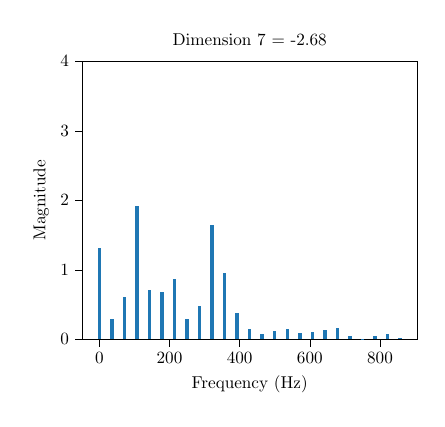
\begin{tikzpicture}[scale=0.62]

\definecolor{darkgray176}{RGB}{176,176,176}
\definecolor{steelblue31119180}{RGB}{31,119,180}

\begin{axis}[
tick align=outside,
tick pos=left,
x grid style={darkgray176},
xlabel={Frequency (Hz)},
xmin=-48.3571428571429, xmax=905.5,
xtick style={color=black},
y grid style={darkgray176},
ylabel={Magnitude},
ymin=0, ymax=4,
title={Dimension 7 = -2.68},
ytick style={color=black}
]
\draw[draw=none,fill=steelblue31119180] (axis cs:-5,0) rectangle (axis cs:5,1.31270937714726);
\draw[draw=none,fill=steelblue31119180] (axis cs:30.7142857142857,0) rectangle (axis cs:40.7142857142857,0.288125975872221);
\draw[draw=none,fill=steelblue31119180] (axis cs:66.4285714285714,0) rectangle (axis cs:76.4285714285714,0.616790952368152);
\draw[draw=none,fill=steelblue31119180] (axis cs:102.142857142857,0) rectangle (axis cs:112.142857142857,1.92312523138079);
\draw[draw=none,fill=steelblue31119180] (axis cs:137.857142857143,0) rectangle (axis cs:147.857142857143,0.707237007629874);
\draw[draw=none,fill=steelblue31119180] (axis cs:173.571428571429,0) rectangle (axis cs:183.571428571429,0.677698119881814);
\draw[draw=none,fill=steelblue31119180] (axis cs:209.285714285714,0) rectangle (axis cs:219.285714285714,0.862386040544995);
\draw[draw=none,fill=steelblue31119180] (axis cs:245,0) rectangle (axis cs:255,0.298711415685218);
\draw[draw=none,fill=steelblue31119180] (axis cs:280.714285714286,0) rectangle (axis cs:290.714285714286,0.483968708976862);
\draw[draw=none,fill=steelblue31119180] (axis cs:316.428571428571,0) rectangle (axis cs:326.428571428571,1.65269155101225);
\draw[draw=none,fill=steelblue31119180] (axis cs:352.142857142857,0) rectangle (axis cs:362.142857142857,0.951122100407993);
\draw[draw=none,fill=steelblue31119180] (axis cs:387.857142857143,0) rectangle (axis cs:397.857142857143,0.377021033569998);
\draw[draw=none,fill=steelblue31119180] (axis cs:423.571428571429,0) rectangle (axis cs:433.571428571429,0.156449857538637);
\draw[draw=none,fill=steelblue31119180] (axis cs:459.285714285714,0) rectangle (axis cs:469.285714285714,0.0846393619854383);
\draw[draw=none,fill=steelblue31119180] (axis cs:495,0) rectangle (axis cs:505,0.118818944486802);
\draw[draw=none,fill=steelblue31119180] (axis cs:530.714285714286,0) rectangle (axis cs:540.714285714286,0.143214948815801);
\draw[draw=none,fill=steelblue31119180] (axis cs:566.428571428571,0) rectangle (axis cs:576.428571428571,0.0949080699867579);
\draw[draw=none,fill=steelblue31119180] (axis cs:602.142857142857,0) rectangle (axis cs:612.142857142857,0.10757439472035);
\draw[draw=none,fill=steelblue31119180] (axis cs:637.857142857143,0) rectangle (axis cs:647.857142857143,0.131395993038413);
\draw[draw=none,fill=steelblue31119180] (axis cs:673.571428571429,0) rectangle (axis cs:683.571428571429,0.160127533802761);
\draw[draw=none,fill=steelblue31119180] (axis cs:709.285714285714,0) rectangle (axis cs:719.285714285714,0.0535699464522896);
\draw[draw=none,fill=steelblue31119180] (axis cs:745,0) rectangle (axis cs:755,0.00967304476823895);
\draw[draw=none,fill=steelblue31119180] (axis cs:780.714285714286,0) rectangle (axis cs:790.714285714286,0.0422317493349039);
\draw[draw=none,fill=steelblue31119180] (axis cs:816.428571428571,0) rectangle (axis cs:826.428571428571,0.0743497564419976);
\draw[draw=none,fill=steelblue31119180] (axis cs:852.142857142857,0) rectangle (axis cs:862.142857142857,0.0273048386393424);
\end{axis}

\end{tikzpicture}

	\end{subfigure}\hfill
	\begin{subfigure}{0.3\textwidth}
		\centering
		% This file was created with tikzplotlib v0.10.1.
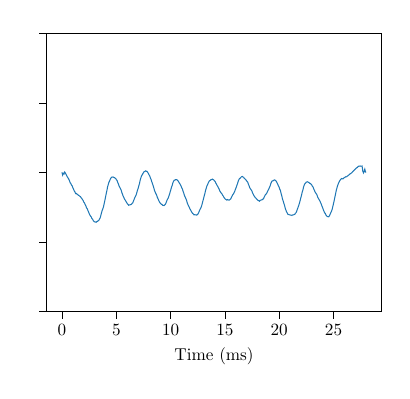
\begin{tikzpicture}[scale=0.62]

\definecolor{darkgray176}{RGB}{176,176,176}
\definecolor{steelblue31119180}{RGB}{31,119,180}

\begin{axis}[
yticklabel={\empty},
tick align=outside,
tick pos=left,
x grid style={darkgray176},
xlabel={Time (ms)},
xmin=-1.4, xmax=29.4,
xtick style={color=black},
y grid style={darkgray176},
% ylabel={Amplitude},
ymin=-0.1, ymax=0.1,
ytick style={color=black}
]
\addplot [semithick, steelblue31119180]
table {%
0 0
0.0626398210290828 -0.00193993691605009
0.125279642058166 -0.000697388132446564
0.187919463087248 -0.00111275092517369
0.250559284116331 0.00024235098553984
0.313199105145414 -0.000513447461112232
0.375838926174497 -0.00148002097020613
0.438478747203579 -0.00236590096614505
0.501118568232662 -0.00338719153914276
0.563758389261745 -0.0040478758738945
0.626398210290828 -0.00489145892378468
0.68903803131991 -0.00597273225852307
0.751677852348993 -0.0075518943669412
0.814317673378076 -0.00804388824375284
0.876957494407159 -0.00911086484564831
0.939597315436242 -0.00976522177482811
1.00223713646532 -0.0111615252149785
1.06487695749441 -0.0120892122812919
1.12751677852349 -0.0133643534484526
1.19015659955257 -0.0140450388668167
1.25279642058166 -0.0152411321678118
1.31543624161074 -0.0152015755478068
1.37807606263982 -0.0156972490801107
1.4407158836689 -0.0158916462787846
1.50335570469799 -0.0164657530043549
1.56599552572707 -0.0166319236784373
1.62863534675615 -0.0171322892138722
1.69127516778523 -0.0173743133176893
1.75391498881432 -0.0181628179505167
1.8165548098434 -0.0186722927520539
1.87919463087248 -0.0195240025227302
1.94183445190157 -0.0201793634176454
2.00447427293065 -0.0213767018969227
2.06711409395973 -0.0218668722441332
2.12975391498881 -0.0232046467170819
2.1923937360179 -0.0239699781816078
2.25503355704698 -0.0254819174265902
2.31767337807606 -0.0260842469514616
2.38031319910515 -0.02732341299021
2.44295302013423 -0.0283705943307821
2.50559284116331 -0.0296850969152363
2.56823266219239 -0.0306688831281542
2.63087248322148 -0.0315327634222355
2.69351230425056 -0.0320830301525409
2.75615212527964 -0.0332634595391534
2.81879194630872 -0.0337594674162617
2.88143176733781 -0.0346627948093134
2.94407158836689 -0.0353023716492341
3.00671140939597 -0.0356445175864352
3.06935123042506 -0.035673768940888
3.13199105145414 -0.0359154810516426
3.19463087248322 -0.035473047324375
3.2572706935123 -0.0353451175052648
3.31991051454139 -0.034851632399747
3.38255033557047 -0.0345895809540213
3.44519015659955 -0.0336693489436535
3.50782997762864 -0.0329108504115935
3.57046979865772 -0.0311585394228065
3.6331096196868 -0.0292167303671173
3.69574944071588 -0.0274955162390967
3.75838926174497 -0.0262148996452557
3.82102908277405 -0.0247058035468295
3.88366890380313 -0.0225165513962907
3.94630872483221 -0.0201710773344408
4.0089485458613 -0.0177496855815985
4.07158836689038 -0.015311727462799
4.13422818791946 -0.0130772745024238
4.19686800894855 -0.0104869296586754
4.25950782997763 -0.00871839223667079
4.32214765100671 -0.00709854418899389
4.38478747203579 -0.00616015045709858
4.44742729306488 -0.00491042862702536
4.51006711409396 -0.00406632385522927
4.57270693512304 -0.00346006396782878
4.63534675615213 -0.00342682171487968
4.69798657718121 -0.00326321851587135
4.76062639821029 -0.0036356184669089
4.82326621923937 -0.00375522114961539
4.88590604026846 -0.00417020489405466
4.94854586129754 -0.00445070286475172
5.01118568232662 -0.00530394186709551
5.0738255033557 -0.00580074416235989
5.13646532438479 -0.00734688157228216
5.19910514541387 -0.00843495169917009
5.26174496644295 -0.00992326142778933
5.32438478747204 -0.0108189789840839
5.38702460850112 -0.0118006604079832
5.4496644295302 -0.012858154283424
5.51230425055928 -0.0146084608847663
5.57494407158837 -0.0158316910629404
5.63758389261745 -0.017210534067462
5.70022371364653 -0.0182066267768809
5.76286353467562 -0.019341929859463
5.8255033557047 -0.0199633272827272
5.88814317673378 -0.0208683198805423
5.95078299776286 -0.0216582978656828
6.01342281879195 -0.022514550627878
6.07606263982103 -0.0229377234917159
6.13870246085011 -0.0236546001053296
6.2013422818792 -0.0234269479902199
6.26398210290828 -0.0233680328991789
6.32662192393736 -0.0231993186018811
6.38926174496644 -0.0230197730230405
6.45190156599553 -0.0223188432646078
6.51454138702461 -0.0219767539568195
6.57718120805369 -0.020686269068978
6.63982102908277 -0.0194335101959889
6.70246085011186 -0.0182000818543586
6.76510067114094 -0.0172540410328031
6.82774049217002 -0.016209368493983
6.89038031319911 -0.0145123920359668
6.95302013422819 -0.0128312964904928
7.01565995525727 -0.011369697843372
7.07829977628635 -0.00948762195497351
7.14093959731544 -0.00777829895358558
7.20357941834452 -0.00547778635167035
7.2662192393736 -0.00382289449815582
7.32885906040269 -0.00239693011538494
7.39149888143177 -0.001753756326417
7.45413870246085 -0.000781532301998778
7.51677852348993 6.73212836052733e-05
7.57941834451902 0.000587434764176407
7.6420581655481 0.000659656592163462
7.70469798657718 0.0011229761594894
7.76733780760626 0.000801310005704027
7.82997762863535 0.000698161930245841
7.89261744966443 -3.1259598447974e-05
7.95525727069351 -0.000749898274372888
8.0178970917226 -0.00186771298164889
8.08053691275168 -0.00256872730917179
8.14317673378076 -0.00407967935222507
8.20581655480984 -0.00523308175772228
8.26845637583893 -0.00684347297471242
8.33109619686801 -0.00807858403497094
8.39373601789709 -0.00967644710068735
8.45637583892617 -0.0112190790124388
8.51901565995526 -0.0130481103110133
8.58165548098434 -0.0142187896815922
8.64429530201342 -0.0153381289639229
8.70693512304251 -0.0162461492914281
8.76957494407159 -0.0178199395312359
8.83221476510067 -0.0188130948492545
8.89485458612975 -0.0201093304727302
8.95749440715884 -0.0210614237784339
9.02013422818792 -0.0218487176919143
9.082774049217 -0.0223928749461302
9.14541387024608 -0.0229616805836058
9.20805369127517 -0.0230043411204879
9.27069351230425 -0.0237804200475248
9.33333333333333 -0.0237110909074545
9.39597315436242 -0.0239102192248074
9.4586129753915 -0.0234278298964436
9.52125279642058 -0.0228990960941219
9.58389261744967 -0.0218231376360527
9.64653243847875 -0.0205061491703827
9.70917225950783 -0.0193424955160426
9.77181208053691 -0.018616105261065
9.834451901566 -0.0172838850146872
9.89709172259508 -0.0157916663439582
9.95973154362416 -0.0140185877930798
10.0223713646532 -0.0123708326644545
10.0850111856823 -0.0106744820552084
10.1476510067114 -0.00930849950285566
10.2102908277405 -0.00748266152812531
10.2729306487696 -0.00644440207655398
10.3355704697987 -0.00563968386776095
10.3982102908277 -0.00555548336881919
10.4608501118568 -0.00516599532991848
10.5234899328859 -0.0051542442767012
10.586129753915 -0.00529719335370816
10.6487695749441 -0.00593067748134568
10.7114093959732 -0.00634356388734691
10.7740492170022 -0.00736922608850986
10.8366890380313 -0.00803187458257147
10.8993288590604 -0.0089733005195056
10.9619686800895 -0.00978573921117807
11.0246085011186 -0.0111731671471924
11.0872483221477 -0.0119811839192806
11.1498881431767 -0.0137315380180742
11.2125279642058 -0.0149477422987455
11.2751677852349 -0.0166889945820174
11.337807606264 -0.0176660706157852
11.4004474272931 -0.0188565955391066
11.4630872483221 -0.0200510227040156
11.5257270693512 -0.0218445007633043
11.5883668903803 -0.0230041039145033
11.6510067114094 -0.0241762147278794
11.7136465324385 -0.0250530869718766
11.7762863534676 -0.0262797192714158
11.8389261744966 -0.027023786778918
11.9015659955257 -0.0280513898563265
11.9642058165548 -0.0288587481833544
12.0268456375839 -0.0295683772446925
12.089485458613 -0.0299139131960653
12.1521252796421 -0.0305846930675259
12.2147651006711 -0.0303976354407984
12.2774049217002 -0.0306569234711812
12.3400447427293 -0.0306414825179233
12.4026845637584 -0.0307158210608583
12.4653243847875 -0.0302266703306029
12.5279642058166 -0.0299377874815024
12.5906040268456 -0.0288169970173364
12.6532438478747 -0.0275692523850891
12.7158836689038 -0.0264562012115181
12.7785234899329 -0.0256634560857443
12.841163310962 -0.0244389498143788
12.9038031319911 -0.0226962687010133
12.9664429530201 -0.0207448930998377
13.0290827740492 -0.0189703644797106
13.0917225950783 -0.0169095892096626
13.1543624161074 -0.0151532614266112
13.2170022371365 -0.0129474857509536
13.2796420581655 -0.0113705251078378
13.3422818791946 -0.00967341267672561
13.4049217002237 -0.00875322164455116
13.4675615212528 -0.00757922379037478
13.5302013422819 -0.00659251304330842
13.592841163311 -0.00594735833122426
13.65548098434 -0.00570734011496873
13.7181208053691 -0.00515767018116961
13.7807606263982 -0.00519810113180804
13.8434004474273 -0.00482528749228324
13.9060402684564 -0.00515122189742807
13.9686800894855 -0.00544539820277851
14.0313199105145 -0.00606688503300984
14.0939597315436 -0.00646338295566556
14.1565995525727 -0.00763518456994687
14.2192393736018 -0.00843569395076109
14.2818791946309 -0.00947208871327391
14.34451901566 -0.0101807585123601
14.407158836689 -0.0111817509098441
14.4697986577181 -0.0120870489814638
14.5324384787472 -0.0134959457654681
14.5950782997763 -0.0141432432695323
14.6577181208054 -0.0148773754278085
14.7203579418345 -0.0154101146672596
14.7829977628635 -0.0163902547522979
14.8456375838926 -0.0170291740784809
14.9082774049217 -0.0179558711488975
14.9709172259508 -0.0186465589717131
15.0335570469799 -0.0192331361065575
15.0961968680089 -0.0195358479833043
15.158836689038 -0.0198954767078761
15.2214765100671 -0.0195587890710207
15.2841163310962 -0.0198893158277809
15.3467561521253 -0.0198336920307187
15.4093959731544 -0.019957424197721
15.4720357941834 -0.0194759885436737
15.5346756152125 -0.0190920362861564
15.5973154362416 -0.0180706887212176
15.6599552572707 -0.0169706257722722
15.7225950782998 -0.0159926750453427
15.7852348993289 -0.0154632865232509
15.8478747203579 -0.0145415439076672
15.910514541387 -0.0134155520069219
15.9731543624161 -0.0120827655164187
16.0357941834452 -0.0108127846263799
16.0984340044743 -0.00937753682018527
16.1610738255034 -0.0080538707716553
16.2237136465324 -0.00633208294892871
16.2863534675615 -0.00529039064234735
16.3489932885906 -0.00436794674086491
16.4116331096197 -0.00420468906253176
16.4742729306488 -0.0035372096170115
16.5369127516779 -0.00309298029982004
16.5995525727069 -0.00297285403256248
16.662192393736 -0.00334789148913134
16.7248322147651 -0.00356254867909339
16.7874720357942 -0.00435261607120101
16.8501118568233 -0.00472985238036853
16.9127516778523 -0.0053461461559238
16.9753914988814 -0.00567663938507138
17.0380313199105 -0.00658133582230782
17.1006711409396 -0.00707126775093927
17.1633109619687 -0.00855818980892233
17.2259507829978 -0.00963812948973387
17.2885906040268 -0.0111377743454087
17.3512304250559 -0.0117959981259184
17.413870246085 -0.0125579870737239
17.4765100671141 -0.0133017546953571
17.5391498881432 -0.0146937936094383
17.6017897091723 -0.0156262248329468
17.6644295302013 -0.0166750974553143
17.7270693512304 -0.0173641191420439
17.7897091722595 -0.0181859511532039
17.8523489932886 -0.0185211233469664
17.9149888143177 -0.0191185392139342
17.9776286353468 -0.0196192912482375
18.0402684563758 -0.0201465971517883
18.1029082774049 -0.0202752597405006
18.165548098434 -0.0207546639987486
18.2281879194631 -0.0202718090090976
18.2908277404922 -0.0199718117563917
18.3534675615213 -0.0198644418144386
18.4161073825503 -0.01982115804149
18.4787472035794 -0.0192898742779589
18.5413870246085 -0.0190784383515184
18.6040268456376 -0.0180081292961868
18.6666666666667 -0.0169898476451635
18.7293064876958 -0.0160652905727593
18.7919463087248 -0.0155984235977466
18.8545861297539 -0.0149188462719821
18.917225950783 -0.0138154529135099
18.9798657718121 -0.0127515262117822
19.0425055928412 -0.0119236599803971
19.1051454138702 -0.0107432210992947
19.1677852348993 -0.00963751154157939
19.2304250559284 -0.00792205298706989
19.2930648769575 -0.00688576142009873
19.3557046979866 -0.00610579497137126
19.4183445190157 -0.0061797442214701
19.4809843400447 -0.00575651343436849
19.5436241610738 -0.00549986924751093
19.6062639821029 -0.00550226312155691
19.668903803132 -0.00602696132189875
19.7315436241611 -0.00635458142090364
19.7941834451902 -0.00754223414540491
19.8568232662192 -0.0084792148796904
19.9194630872483 -0.00964791891508854
19.9821029082774 -0.0105099868554397
20.0447427293065 -0.0120551966680776
20.1073825503356 -0.0130137496271589
20.1700223713647 -0.0152044488717146
20.2326621923937 -0.0168635845809375
20.2953020134228 -0.019133672555721
20.3579418344519 -0.0205623124469847
20.420581655481 -0.0221308947309552
20.4832214765101 -0.0235966664532687
20.5458612975392 -0.0256366451089614
20.6085011185682 -0.0270639085054598
20.6711409395973 -0.0283343148286511
20.7337807606264 -0.0291837782492774
20.7964205816555 -0.0301544365391835
20.8590604026846 -0.0303579606990886
20.9217002237136 -0.0305262249863188
20.9843400447427 -0.0306423743249186
21.0469798657718 -0.0307146397438025
21.1096196868009 -0.0307650097689573
21.17225950783 -0.0310371947543533
21.2348993288591 -0.0305777494889378
21.2975391498881 -0.0306150344319192
21.3601789709172 -0.0303580903591926
21.4228187919463 -0.0302442793903135
21.4854586129754 -0.0294810385637035
21.5480984340045 -0.0290137161719519
21.6107382550336 -0.0278098889870332
21.6733780760626 -0.0264089604177131
21.7360178970917 -0.0250087135765176
21.7986577181208 -0.0237058942524979
21.8612975391499 -0.0220596348279275
21.923937360179 -0.02028223028369
21.9865771812081 -0.0182890103592369
22.0492170022371 -0.0164573208847702
22.1118568232662 -0.0143455547724394
22.1744966442953 -0.0127747641413804
22.2371364653244 -0.010639312633332
22.2997762863535 -0.00914210952418363
22.3624161073826 -0.00808671373723937
22.4250559284116 -0.00765494831006399
22.4876957494407 -0.00705658045016079
22.5503355704698 -0.00685571037832923
22.6129753914989 -0.00677605473355159
22.675615212528 -0.00717133541760229
22.738255033557 -0.00729907692828834
22.8008948545861 -0.00784356573334076
22.8635346756152 -0.00799461079748885
22.9261744966443 -0.00850925071402484
22.9888143176734 -0.00898205096389623
23.0514541387025 -0.00996084994442711
23.1140939597315 -0.0106121865944974
23.1767337807606 -0.0119826560777506
23.2393736017897 -0.0128798367418099
23.3020134228188 -0.01422062497461
23.3646532438479 -0.0148710731429442
23.427293064877 -0.0156335985325527
23.489932885906 -0.0165303014281312
23.5525727069351 -0.018088021696914
23.6152125279642 -0.0188820565231894
23.6778523489933 -0.0197612943265262
23.7404921700224 -0.0205219524143726
23.8031319910515 -0.0217698877864836
23.8657718120805 -0.0227528209079232
23.9284116331096 -0.024208398373335
23.9910514541387 -0.0253864640632532
24.0536912751678 -0.0268292097662319
24.1163310961969 -0.0279409261732893
24.1789709172259 -0.0291731259191796
24.241610738255 -0.0295585168888105
24.3042505592841 -0.0308126008525591
24.3668903803132 -0.031327838678188
24.4295302013423 -0.0318774218177235
24.4921700223714 -0.0318811046422128
24.5548098434004 -0.0319863388802381
24.6174496644295 -0.0312568510463774
24.6800894854586 -0.0302467762098816
24.7427293064877 -0.0290509528111691
24.8053691275168 -0.0280506531364166
24.8680089485459 -0.0266603137047699
24.9306487695749 -0.0246157685932297
24.993288590604 -0.0225176575324879
25.0559284116331 -0.0203431202786281
25.1185682326622 -0.0178945301813167
25.1812080536913 -0.0156796480335245
25.2438478747204 -0.0131607170047976
25.3064876957494 -0.0113573145908897
25.3691275167785 -0.00954080660571188
25.4317673378076 -0.0083261649030567
25.4944071588367 -0.00708915283215926
25.5570469798658 -0.00624982667649352
25.6196868008949 -0.00537700829839946
25.6823266219239 -0.00494568711209217
25.744966442953 -0.00445876410543519
25.8076062639821 -0.00463843895684953
25.8702460850112 -0.00463734595917615
25.9328859060403 -0.00417199610863756
25.9955257270694 -0.00376390583263148
26.0581655480984 -0.00351306192276862
26.1208053691275 -0.00316015437195365
26.1834451901566 -0.00319486327669365
26.2460850111857 -0.0028069100573959
26.3087248322148 -0.00251574174269734
26.3713646532438 -0.00206075192447877
26.4340044742729 -0.00175063678332223
26.496644295302 -0.00115453855653337
26.5592841163311 -0.000961863192035849
26.6219239373602 -0.000519481618832422
26.6845637583893 -0.000253477640099975
26.7472035794183 0.000386290302212607
26.8098434004474 0.000813860121189346
26.8724832214765 0.00136720877915821
26.9351230425056 0.00177161288041396
26.9977628635347 0.0023945276094163
27.0604026845638 0.0027713477986571
27.1230425055928 0.00326533768101027
27.1856823266219 0.00345150310071123
27.248322147651 0.00407087321599458
27.3109619686801 0.00446927401193436
27.3736017897092 0.00457032027360577
27.4362416107383 0.00441366212830047
27.4988814317673 0.00459057578954521
27.5615212527964 0.00445979537329818
27.6241610738255 0.00456084163496958
27.6868008948546 0.00105147996304819
27.7494407158837 -0.000385981415642188
27.8120805369128 0.00072438754891389
27.8747203579418 0.00228477716945962
27.9373601789709 0.00025185048830189
28 0
};
\end{axis}

\end{tikzpicture}

	\end{subfigure}\hfill
	\begin{subfigure}{0.3\textwidth}
		\centering
		% This file was created with tikzplotlib v0.10.1.
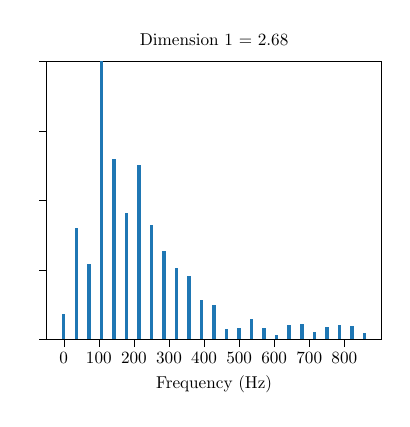
\begin{tikzpicture}[scale=0.62]

\definecolor{darkgray176}{RGB}{176,176,176}
\definecolor{steelblue31119180}{RGB}{31,119,180}

\begin{axis}[
yticklabel={\empty},
tick align=outside,
tick pos=left,
x grid style={darkgray176},
xlabel={Frequency (Hz)},
xmin=-48.3571428571429, xmax=905.5,
xtick style={color=black},
xtick={0, 100, 200, 300, 400, 500, 600, 700, 800}, % Set explicit tick positions
y grid style={darkgray176},
%ylabel={Magnitude},
ymin=0, ymax=4,
title={Dimension 1 = 2.68},
ytick style={color=black}
]
\draw[draw=none,fill=steelblue31119180] (axis cs:-5,0) rectangle (axis cs:5,0.363293109461665);
\draw[draw=none,fill=steelblue31119180] (axis cs:30.7142857142857,0) rectangle (axis cs:40.7142857142857,1.59671692845371);
\draw[draw=none,fill=steelblue31119180] (axis cs:66.4285714285714,0) rectangle (axis cs:76.4285714285714,1.08375129075336);
\draw[draw=none,fill=steelblue31119180] (axis cs:102.142857142857,0) rectangle (axis cs:112.142857142857,5.72028640718505);
\draw[draw=none,fill=steelblue31119180] (axis cs:137.857142857143,0) rectangle (axis cs:147.857142857143,2.60109171070077);
\draw[draw=none,fill=steelblue31119180] (axis cs:173.571428571429,0) rectangle (axis cs:183.571428571429,1.82230187959835);
\draw[draw=none,fill=steelblue31119180] (axis cs:209.285714285714,0) rectangle (axis cs:219.285714285714,2.50466396839656);
\draw[draw=none,fill=steelblue31119180] (axis cs:245,0) rectangle (axis cs:255,1.64154431128106);
\draw[draw=none,fill=steelblue31119180] (axis cs:280.714285714286,0) rectangle (axis cs:290.714285714286,1.2779936763853);
\draw[draw=none,fill=steelblue31119180] (axis cs:316.428571428571,0) rectangle (axis cs:326.428571428571,1.02566988726104);
\draw[draw=none,fill=steelblue31119180] (axis cs:352.142857142857,0) rectangle (axis cs:362.142857142857,0.906444113984638);
\draw[draw=none,fill=steelblue31119180] (axis cs:387.857142857143,0) rectangle (axis cs:397.857142857143,0.567573738688084);
\draw[draw=none,fill=steelblue31119180] (axis cs:423.571428571429,0) rectangle (axis cs:433.571428571429,0.497884322563813);
\draw[draw=none,fill=steelblue31119180] (axis cs:459.285714285714,0) rectangle (axis cs:469.285714285714,0.143370970638671);
\draw[draw=none,fill=steelblue31119180] (axis cs:495,0) rectangle (axis cs:505,0.158030205491621);
\draw[draw=none,fill=steelblue31119180] (axis cs:530.714285714286,0) rectangle (axis cs:540.714285714286,0.287791882784369);
\draw[draw=none,fill=steelblue31119180] (axis cs:566.428571428571,0) rectangle (axis cs:576.428571428571,0.164560600100172);
\draw[draw=none,fill=steelblue31119180] (axis cs:602.142857142857,0) rectangle (axis cs:612.142857142857,0.0653538748355305);
\draw[draw=none,fill=steelblue31119180] (axis cs:637.857142857143,0) rectangle (axis cs:647.857142857143,0.209706204538538);
\draw[draw=none,fill=steelblue31119180] (axis cs:673.571428571429,0) rectangle (axis cs:683.571428571429,0.216581742305538);
\draw[draw=none,fill=steelblue31119180] (axis cs:709.285714285714,0) rectangle (axis cs:719.285714285714,0.104565114650486);
\draw[draw=none,fill=steelblue31119180] (axis cs:745,0) rectangle (axis cs:755,0.18370350932939);
\draw[draw=none,fill=steelblue31119180] (axis cs:780.714285714286,0) rectangle (axis cs:790.714285714286,0.206670350113575);
\draw[draw=none,fill=steelblue31119180] (axis cs:816.428571428571,0) rectangle (axis cs:826.428571428571,0.196489132073225);
\draw[draw=none,fill=steelblue31119180] (axis cs:852.142857142857,0) rectangle (axis cs:862.142857142857,0.0885177801919891);
\end{axis}

\end{tikzpicture}

	\end{subfigure}
	
	\vspace{0.5cm} % Adjust vertical spacing between rows
	
	\begin{subfigure}{0.36\textwidth}
		\centering
		% This file was created with tikzplotlib v0.10.1.
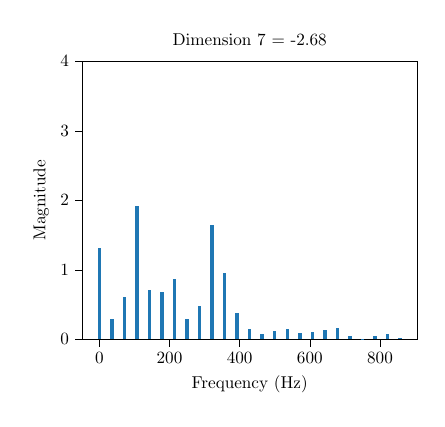
\begin{tikzpicture}[scale=0.62]

\definecolor{darkgray176}{RGB}{176,176,176}
\definecolor{steelblue31119180}{RGB}{31,119,180}

\begin{axis}[
tick align=outside,
tick pos=left,
x grid style={darkgray176},
xlabel={Frequency (Hz)},
xmin=-48.3571428571429, xmax=905.5,
xtick style={color=black},
y grid style={darkgray176},
ylabel={Magnitude},
ymin=0, ymax=4,
title={Dimension 7 = -2.68},
ytick style={color=black}
]
\draw[draw=none,fill=steelblue31119180] (axis cs:-5,0) rectangle (axis cs:5,1.31270937714726);
\draw[draw=none,fill=steelblue31119180] (axis cs:30.7142857142857,0) rectangle (axis cs:40.7142857142857,0.288125975872221);
\draw[draw=none,fill=steelblue31119180] (axis cs:66.4285714285714,0) rectangle (axis cs:76.4285714285714,0.616790952368152);
\draw[draw=none,fill=steelblue31119180] (axis cs:102.142857142857,0) rectangle (axis cs:112.142857142857,1.92312523138079);
\draw[draw=none,fill=steelblue31119180] (axis cs:137.857142857143,0) rectangle (axis cs:147.857142857143,0.707237007629874);
\draw[draw=none,fill=steelblue31119180] (axis cs:173.571428571429,0) rectangle (axis cs:183.571428571429,0.677698119881814);
\draw[draw=none,fill=steelblue31119180] (axis cs:209.285714285714,0) rectangle (axis cs:219.285714285714,0.862386040544995);
\draw[draw=none,fill=steelblue31119180] (axis cs:245,0) rectangle (axis cs:255,0.298711415685218);
\draw[draw=none,fill=steelblue31119180] (axis cs:280.714285714286,0) rectangle (axis cs:290.714285714286,0.483968708976862);
\draw[draw=none,fill=steelblue31119180] (axis cs:316.428571428571,0) rectangle (axis cs:326.428571428571,1.65269155101225);
\draw[draw=none,fill=steelblue31119180] (axis cs:352.142857142857,0) rectangle (axis cs:362.142857142857,0.951122100407993);
\draw[draw=none,fill=steelblue31119180] (axis cs:387.857142857143,0) rectangle (axis cs:397.857142857143,0.377021033569998);
\draw[draw=none,fill=steelblue31119180] (axis cs:423.571428571429,0) rectangle (axis cs:433.571428571429,0.156449857538637);
\draw[draw=none,fill=steelblue31119180] (axis cs:459.285714285714,0) rectangle (axis cs:469.285714285714,0.0846393619854383);
\draw[draw=none,fill=steelblue31119180] (axis cs:495,0) rectangle (axis cs:505,0.118818944486802);
\draw[draw=none,fill=steelblue31119180] (axis cs:530.714285714286,0) rectangle (axis cs:540.714285714286,0.143214948815801);
\draw[draw=none,fill=steelblue31119180] (axis cs:566.428571428571,0) rectangle (axis cs:576.428571428571,0.0949080699867579);
\draw[draw=none,fill=steelblue31119180] (axis cs:602.142857142857,0) rectangle (axis cs:612.142857142857,0.10757439472035);
\draw[draw=none,fill=steelblue31119180] (axis cs:637.857142857143,0) rectangle (axis cs:647.857142857143,0.131395993038413);
\draw[draw=none,fill=steelblue31119180] (axis cs:673.571428571429,0) rectangle (axis cs:683.571428571429,0.160127533802761);
\draw[draw=none,fill=steelblue31119180] (axis cs:709.285714285714,0) rectangle (axis cs:719.285714285714,0.0535699464522896);
\draw[draw=none,fill=steelblue31119180] (axis cs:745,0) rectangle (axis cs:755,0.00967304476823895);
\draw[draw=none,fill=steelblue31119180] (axis cs:780.714285714286,0) rectangle (axis cs:790.714285714286,0.0422317493349039);
\draw[draw=none,fill=steelblue31119180] (axis cs:816.428571428571,0) rectangle (axis cs:826.428571428571,0.0743497564419976);
\draw[draw=none,fill=steelblue31119180] (axis cs:852.142857142857,0) rectangle (axis cs:862.142857142857,0.0273048386393424);
\end{axis}

\end{tikzpicture}

	\end{subfigure}\hfill
	\begin{subfigure}{0.3\textwidth}
		\centering
		% This file was created with tikzplotlib v0.10.1.
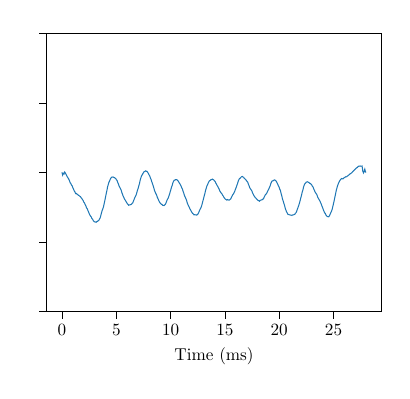
\begin{tikzpicture}[scale=0.62]

\definecolor{darkgray176}{RGB}{176,176,176}
\definecolor{steelblue31119180}{RGB}{31,119,180}

\begin{axis}[
yticklabel={\empty},
tick align=outside,
tick pos=left,
x grid style={darkgray176},
xlabel={Time (ms)},
xmin=-1.4, xmax=29.4,
xtick style={color=black},
y grid style={darkgray176},
% ylabel={Amplitude},
ymin=-0.1, ymax=0.1,
ytick style={color=black}
]
\addplot [semithick, steelblue31119180]
table {%
0 0
0.0626398210290828 -0.00193993691605009
0.125279642058166 -0.000697388132446564
0.187919463087248 -0.00111275092517369
0.250559284116331 0.00024235098553984
0.313199105145414 -0.000513447461112232
0.375838926174497 -0.00148002097020613
0.438478747203579 -0.00236590096614505
0.501118568232662 -0.00338719153914276
0.563758389261745 -0.0040478758738945
0.626398210290828 -0.00489145892378468
0.68903803131991 -0.00597273225852307
0.751677852348993 -0.0075518943669412
0.814317673378076 -0.00804388824375284
0.876957494407159 -0.00911086484564831
0.939597315436242 -0.00976522177482811
1.00223713646532 -0.0111615252149785
1.06487695749441 -0.0120892122812919
1.12751677852349 -0.0133643534484526
1.19015659955257 -0.0140450388668167
1.25279642058166 -0.0152411321678118
1.31543624161074 -0.0152015755478068
1.37807606263982 -0.0156972490801107
1.4407158836689 -0.0158916462787846
1.50335570469799 -0.0164657530043549
1.56599552572707 -0.0166319236784373
1.62863534675615 -0.0171322892138722
1.69127516778523 -0.0173743133176893
1.75391498881432 -0.0181628179505167
1.8165548098434 -0.0186722927520539
1.87919463087248 -0.0195240025227302
1.94183445190157 -0.0201793634176454
2.00447427293065 -0.0213767018969227
2.06711409395973 -0.0218668722441332
2.12975391498881 -0.0232046467170819
2.1923937360179 -0.0239699781816078
2.25503355704698 -0.0254819174265902
2.31767337807606 -0.0260842469514616
2.38031319910515 -0.02732341299021
2.44295302013423 -0.0283705943307821
2.50559284116331 -0.0296850969152363
2.56823266219239 -0.0306688831281542
2.63087248322148 -0.0315327634222355
2.69351230425056 -0.0320830301525409
2.75615212527964 -0.0332634595391534
2.81879194630872 -0.0337594674162617
2.88143176733781 -0.0346627948093134
2.94407158836689 -0.0353023716492341
3.00671140939597 -0.0356445175864352
3.06935123042506 -0.035673768940888
3.13199105145414 -0.0359154810516426
3.19463087248322 -0.035473047324375
3.2572706935123 -0.0353451175052648
3.31991051454139 -0.034851632399747
3.38255033557047 -0.0345895809540213
3.44519015659955 -0.0336693489436535
3.50782997762864 -0.0329108504115935
3.57046979865772 -0.0311585394228065
3.6331096196868 -0.0292167303671173
3.69574944071588 -0.0274955162390967
3.75838926174497 -0.0262148996452557
3.82102908277405 -0.0247058035468295
3.88366890380313 -0.0225165513962907
3.94630872483221 -0.0201710773344408
4.0089485458613 -0.0177496855815985
4.07158836689038 -0.015311727462799
4.13422818791946 -0.0130772745024238
4.19686800894855 -0.0104869296586754
4.25950782997763 -0.00871839223667079
4.32214765100671 -0.00709854418899389
4.38478747203579 -0.00616015045709858
4.44742729306488 -0.00491042862702536
4.51006711409396 -0.00406632385522927
4.57270693512304 -0.00346006396782878
4.63534675615213 -0.00342682171487968
4.69798657718121 -0.00326321851587135
4.76062639821029 -0.0036356184669089
4.82326621923937 -0.00375522114961539
4.88590604026846 -0.00417020489405466
4.94854586129754 -0.00445070286475172
5.01118568232662 -0.00530394186709551
5.0738255033557 -0.00580074416235989
5.13646532438479 -0.00734688157228216
5.19910514541387 -0.00843495169917009
5.26174496644295 -0.00992326142778933
5.32438478747204 -0.0108189789840839
5.38702460850112 -0.0118006604079832
5.4496644295302 -0.012858154283424
5.51230425055928 -0.0146084608847663
5.57494407158837 -0.0158316910629404
5.63758389261745 -0.017210534067462
5.70022371364653 -0.0182066267768809
5.76286353467562 -0.019341929859463
5.8255033557047 -0.0199633272827272
5.88814317673378 -0.0208683198805423
5.95078299776286 -0.0216582978656828
6.01342281879195 -0.022514550627878
6.07606263982103 -0.0229377234917159
6.13870246085011 -0.0236546001053296
6.2013422818792 -0.0234269479902199
6.26398210290828 -0.0233680328991789
6.32662192393736 -0.0231993186018811
6.38926174496644 -0.0230197730230405
6.45190156599553 -0.0223188432646078
6.51454138702461 -0.0219767539568195
6.57718120805369 -0.020686269068978
6.63982102908277 -0.0194335101959889
6.70246085011186 -0.0182000818543586
6.76510067114094 -0.0172540410328031
6.82774049217002 -0.016209368493983
6.89038031319911 -0.0145123920359668
6.95302013422819 -0.0128312964904928
7.01565995525727 -0.011369697843372
7.07829977628635 -0.00948762195497351
7.14093959731544 -0.00777829895358558
7.20357941834452 -0.00547778635167035
7.2662192393736 -0.00382289449815582
7.32885906040269 -0.00239693011538494
7.39149888143177 -0.001753756326417
7.45413870246085 -0.000781532301998778
7.51677852348993 6.73212836052733e-05
7.57941834451902 0.000587434764176407
7.6420581655481 0.000659656592163462
7.70469798657718 0.0011229761594894
7.76733780760626 0.000801310005704027
7.82997762863535 0.000698161930245841
7.89261744966443 -3.1259598447974e-05
7.95525727069351 -0.000749898274372888
8.0178970917226 -0.00186771298164889
8.08053691275168 -0.00256872730917179
8.14317673378076 -0.00407967935222507
8.20581655480984 -0.00523308175772228
8.26845637583893 -0.00684347297471242
8.33109619686801 -0.00807858403497094
8.39373601789709 -0.00967644710068735
8.45637583892617 -0.0112190790124388
8.51901565995526 -0.0130481103110133
8.58165548098434 -0.0142187896815922
8.64429530201342 -0.0153381289639229
8.70693512304251 -0.0162461492914281
8.76957494407159 -0.0178199395312359
8.83221476510067 -0.0188130948492545
8.89485458612975 -0.0201093304727302
8.95749440715884 -0.0210614237784339
9.02013422818792 -0.0218487176919143
9.082774049217 -0.0223928749461302
9.14541387024608 -0.0229616805836058
9.20805369127517 -0.0230043411204879
9.27069351230425 -0.0237804200475248
9.33333333333333 -0.0237110909074545
9.39597315436242 -0.0239102192248074
9.4586129753915 -0.0234278298964436
9.52125279642058 -0.0228990960941219
9.58389261744967 -0.0218231376360527
9.64653243847875 -0.0205061491703827
9.70917225950783 -0.0193424955160426
9.77181208053691 -0.018616105261065
9.834451901566 -0.0172838850146872
9.89709172259508 -0.0157916663439582
9.95973154362416 -0.0140185877930798
10.0223713646532 -0.0123708326644545
10.0850111856823 -0.0106744820552084
10.1476510067114 -0.00930849950285566
10.2102908277405 -0.00748266152812531
10.2729306487696 -0.00644440207655398
10.3355704697987 -0.00563968386776095
10.3982102908277 -0.00555548336881919
10.4608501118568 -0.00516599532991848
10.5234899328859 -0.0051542442767012
10.586129753915 -0.00529719335370816
10.6487695749441 -0.00593067748134568
10.7114093959732 -0.00634356388734691
10.7740492170022 -0.00736922608850986
10.8366890380313 -0.00803187458257147
10.8993288590604 -0.0089733005195056
10.9619686800895 -0.00978573921117807
11.0246085011186 -0.0111731671471924
11.0872483221477 -0.0119811839192806
11.1498881431767 -0.0137315380180742
11.2125279642058 -0.0149477422987455
11.2751677852349 -0.0166889945820174
11.337807606264 -0.0176660706157852
11.4004474272931 -0.0188565955391066
11.4630872483221 -0.0200510227040156
11.5257270693512 -0.0218445007633043
11.5883668903803 -0.0230041039145033
11.6510067114094 -0.0241762147278794
11.7136465324385 -0.0250530869718766
11.7762863534676 -0.0262797192714158
11.8389261744966 -0.027023786778918
11.9015659955257 -0.0280513898563265
11.9642058165548 -0.0288587481833544
12.0268456375839 -0.0295683772446925
12.089485458613 -0.0299139131960653
12.1521252796421 -0.0305846930675259
12.2147651006711 -0.0303976354407984
12.2774049217002 -0.0306569234711812
12.3400447427293 -0.0306414825179233
12.4026845637584 -0.0307158210608583
12.4653243847875 -0.0302266703306029
12.5279642058166 -0.0299377874815024
12.5906040268456 -0.0288169970173364
12.6532438478747 -0.0275692523850891
12.7158836689038 -0.0264562012115181
12.7785234899329 -0.0256634560857443
12.841163310962 -0.0244389498143788
12.9038031319911 -0.0226962687010133
12.9664429530201 -0.0207448930998377
13.0290827740492 -0.0189703644797106
13.0917225950783 -0.0169095892096626
13.1543624161074 -0.0151532614266112
13.2170022371365 -0.0129474857509536
13.2796420581655 -0.0113705251078378
13.3422818791946 -0.00967341267672561
13.4049217002237 -0.00875322164455116
13.4675615212528 -0.00757922379037478
13.5302013422819 -0.00659251304330842
13.592841163311 -0.00594735833122426
13.65548098434 -0.00570734011496873
13.7181208053691 -0.00515767018116961
13.7807606263982 -0.00519810113180804
13.8434004474273 -0.00482528749228324
13.9060402684564 -0.00515122189742807
13.9686800894855 -0.00544539820277851
14.0313199105145 -0.00606688503300984
14.0939597315436 -0.00646338295566556
14.1565995525727 -0.00763518456994687
14.2192393736018 -0.00843569395076109
14.2818791946309 -0.00947208871327391
14.34451901566 -0.0101807585123601
14.407158836689 -0.0111817509098441
14.4697986577181 -0.0120870489814638
14.5324384787472 -0.0134959457654681
14.5950782997763 -0.0141432432695323
14.6577181208054 -0.0148773754278085
14.7203579418345 -0.0154101146672596
14.7829977628635 -0.0163902547522979
14.8456375838926 -0.0170291740784809
14.9082774049217 -0.0179558711488975
14.9709172259508 -0.0186465589717131
15.0335570469799 -0.0192331361065575
15.0961968680089 -0.0195358479833043
15.158836689038 -0.0198954767078761
15.2214765100671 -0.0195587890710207
15.2841163310962 -0.0198893158277809
15.3467561521253 -0.0198336920307187
15.4093959731544 -0.019957424197721
15.4720357941834 -0.0194759885436737
15.5346756152125 -0.0190920362861564
15.5973154362416 -0.0180706887212176
15.6599552572707 -0.0169706257722722
15.7225950782998 -0.0159926750453427
15.7852348993289 -0.0154632865232509
15.8478747203579 -0.0145415439076672
15.910514541387 -0.0134155520069219
15.9731543624161 -0.0120827655164187
16.0357941834452 -0.0108127846263799
16.0984340044743 -0.00937753682018527
16.1610738255034 -0.0080538707716553
16.2237136465324 -0.00633208294892871
16.2863534675615 -0.00529039064234735
16.3489932885906 -0.00436794674086491
16.4116331096197 -0.00420468906253176
16.4742729306488 -0.0035372096170115
16.5369127516779 -0.00309298029982004
16.5995525727069 -0.00297285403256248
16.662192393736 -0.00334789148913134
16.7248322147651 -0.00356254867909339
16.7874720357942 -0.00435261607120101
16.8501118568233 -0.00472985238036853
16.9127516778523 -0.0053461461559238
16.9753914988814 -0.00567663938507138
17.0380313199105 -0.00658133582230782
17.1006711409396 -0.00707126775093927
17.1633109619687 -0.00855818980892233
17.2259507829978 -0.00963812948973387
17.2885906040268 -0.0111377743454087
17.3512304250559 -0.0117959981259184
17.413870246085 -0.0125579870737239
17.4765100671141 -0.0133017546953571
17.5391498881432 -0.0146937936094383
17.6017897091723 -0.0156262248329468
17.6644295302013 -0.0166750974553143
17.7270693512304 -0.0173641191420439
17.7897091722595 -0.0181859511532039
17.8523489932886 -0.0185211233469664
17.9149888143177 -0.0191185392139342
17.9776286353468 -0.0196192912482375
18.0402684563758 -0.0201465971517883
18.1029082774049 -0.0202752597405006
18.165548098434 -0.0207546639987486
18.2281879194631 -0.0202718090090976
18.2908277404922 -0.0199718117563917
18.3534675615213 -0.0198644418144386
18.4161073825503 -0.01982115804149
18.4787472035794 -0.0192898742779589
18.5413870246085 -0.0190784383515184
18.6040268456376 -0.0180081292961868
18.6666666666667 -0.0169898476451635
18.7293064876958 -0.0160652905727593
18.7919463087248 -0.0155984235977466
18.8545861297539 -0.0149188462719821
18.917225950783 -0.0138154529135099
18.9798657718121 -0.0127515262117822
19.0425055928412 -0.0119236599803971
19.1051454138702 -0.0107432210992947
19.1677852348993 -0.00963751154157939
19.2304250559284 -0.00792205298706989
19.2930648769575 -0.00688576142009873
19.3557046979866 -0.00610579497137126
19.4183445190157 -0.0061797442214701
19.4809843400447 -0.00575651343436849
19.5436241610738 -0.00549986924751093
19.6062639821029 -0.00550226312155691
19.668903803132 -0.00602696132189875
19.7315436241611 -0.00635458142090364
19.7941834451902 -0.00754223414540491
19.8568232662192 -0.0084792148796904
19.9194630872483 -0.00964791891508854
19.9821029082774 -0.0105099868554397
20.0447427293065 -0.0120551966680776
20.1073825503356 -0.0130137496271589
20.1700223713647 -0.0152044488717146
20.2326621923937 -0.0168635845809375
20.2953020134228 -0.019133672555721
20.3579418344519 -0.0205623124469847
20.420581655481 -0.0221308947309552
20.4832214765101 -0.0235966664532687
20.5458612975392 -0.0256366451089614
20.6085011185682 -0.0270639085054598
20.6711409395973 -0.0283343148286511
20.7337807606264 -0.0291837782492774
20.7964205816555 -0.0301544365391835
20.8590604026846 -0.0303579606990886
20.9217002237136 -0.0305262249863188
20.9843400447427 -0.0306423743249186
21.0469798657718 -0.0307146397438025
21.1096196868009 -0.0307650097689573
21.17225950783 -0.0310371947543533
21.2348993288591 -0.0305777494889378
21.2975391498881 -0.0306150344319192
21.3601789709172 -0.0303580903591926
21.4228187919463 -0.0302442793903135
21.4854586129754 -0.0294810385637035
21.5480984340045 -0.0290137161719519
21.6107382550336 -0.0278098889870332
21.6733780760626 -0.0264089604177131
21.7360178970917 -0.0250087135765176
21.7986577181208 -0.0237058942524979
21.8612975391499 -0.0220596348279275
21.923937360179 -0.02028223028369
21.9865771812081 -0.0182890103592369
22.0492170022371 -0.0164573208847702
22.1118568232662 -0.0143455547724394
22.1744966442953 -0.0127747641413804
22.2371364653244 -0.010639312633332
22.2997762863535 -0.00914210952418363
22.3624161073826 -0.00808671373723937
22.4250559284116 -0.00765494831006399
22.4876957494407 -0.00705658045016079
22.5503355704698 -0.00685571037832923
22.6129753914989 -0.00677605473355159
22.675615212528 -0.00717133541760229
22.738255033557 -0.00729907692828834
22.8008948545861 -0.00784356573334076
22.8635346756152 -0.00799461079748885
22.9261744966443 -0.00850925071402484
22.9888143176734 -0.00898205096389623
23.0514541387025 -0.00996084994442711
23.1140939597315 -0.0106121865944974
23.1767337807606 -0.0119826560777506
23.2393736017897 -0.0128798367418099
23.3020134228188 -0.01422062497461
23.3646532438479 -0.0148710731429442
23.427293064877 -0.0156335985325527
23.489932885906 -0.0165303014281312
23.5525727069351 -0.018088021696914
23.6152125279642 -0.0188820565231894
23.6778523489933 -0.0197612943265262
23.7404921700224 -0.0205219524143726
23.8031319910515 -0.0217698877864836
23.8657718120805 -0.0227528209079232
23.9284116331096 -0.024208398373335
23.9910514541387 -0.0253864640632532
24.0536912751678 -0.0268292097662319
24.1163310961969 -0.0279409261732893
24.1789709172259 -0.0291731259191796
24.241610738255 -0.0295585168888105
24.3042505592841 -0.0308126008525591
24.3668903803132 -0.031327838678188
24.4295302013423 -0.0318774218177235
24.4921700223714 -0.0318811046422128
24.5548098434004 -0.0319863388802381
24.6174496644295 -0.0312568510463774
24.6800894854586 -0.0302467762098816
24.7427293064877 -0.0290509528111691
24.8053691275168 -0.0280506531364166
24.8680089485459 -0.0266603137047699
24.9306487695749 -0.0246157685932297
24.993288590604 -0.0225176575324879
25.0559284116331 -0.0203431202786281
25.1185682326622 -0.0178945301813167
25.1812080536913 -0.0156796480335245
25.2438478747204 -0.0131607170047976
25.3064876957494 -0.0113573145908897
25.3691275167785 -0.00954080660571188
25.4317673378076 -0.0083261649030567
25.4944071588367 -0.00708915283215926
25.5570469798658 -0.00624982667649352
25.6196868008949 -0.00537700829839946
25.6823266219239 -0.00494568711209217
25.744966442953 -0.00445876410543519
25.8076062639821 -0.00463843895684953
25.8702460850112 -0.00463734595917615
25.9328859060403 -0.00417199610863756
25.9955257270694 -0.00376390583263148
26.0581655480984 -0.00351306192276862
26.1208053691275 -0.00316015437195365
26.1834451901566 -0.00319486327669365
26.2460850111857 -0.0028069100573959
26.3087248322148 -0.00251574174269734
26.3713646532438 -0.00206075192447877
26.4340044742729 -0.00175063678332223
26.496644295302 -0.00115453855653337
26.5592841163311 -0.000961863192035849
26.6219239373602 -0.000519481618832422
26.6845637583893 -0.000253477640099975
26.7472035794183 0.000386290302212607
26.8098434004474 0.000813860121189346
26.8724832214765 0.00136720877915821
26.9351230425056 0.00177161288041396
26.9977628635347 0.0023945276094163
27.0604026845638 0.0027713477986571
27.1230425055928 0.00326533768101027
27.1856823266219 0.00345150310071123
27.248322147651 0.00407087321599458
27.3109619686801 0.00446927401193436
27.3736017897092 0.00457032027360577
27.4362416107383 0.00441366212830047
27.4988814317673 0.00459057578954521
27.5615212527964 0.00445979537329818
27.6241610738255 0.00456084163496958
27.6868008948546 0.00105147996304819
27.7494407158837 -0.000385981415642188
27.8120805369128 0.00072438754891389
27.8747203579418 0.00228477716945962
27.9373601789709 0.00025185048830189
28 0
};
\end{axis}

\end{tikzpicture}

	\end{subfigure}\hfill
	\begin{subfigure}{0.3\textwidth}
		\centering
		% This file was created with tikzplotlib v0.10.1.
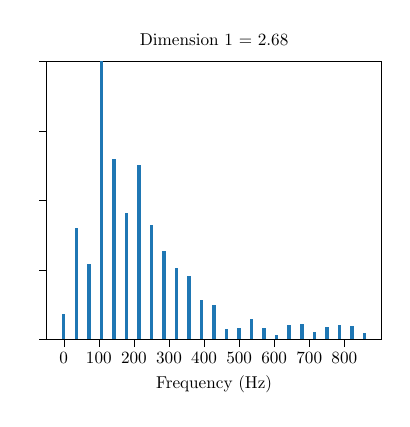
\begin{tikzpicture}[scale=0.62]

\definecolor{darkgray176}{RGB}{176,176,176}
\definecolor{steelblue31119180}{RGB}{31,119,180}

\begin{axis}[
yticklabel={\empty},
tick align=outside,
tick pos=left,
x grid style={darkgray176},
xlabel={Frequency (Hz)},
xmin=-48.3571428571429, xmax=905.5,
xtick style={color=black},
xtick={0, 100, 200, 300, 400, 500, 600, 700, 800}, % Set explicit tick positions
y grid style={darkgray176},
%ylabel={Magnitude},
ymin=0, ymax=4,
title={Dimension 1 = 2.68},
ytick style={color=black}
]
\draw[draw=none,fill=steelblue31119180] (axis cs:-5,0) rectangle (axis cs:5,0.363293109461665);
\draw[draw=none,fill=steelblue31119180] (axis cs:30.7142857142857,0) rectangle (axis cs:40.7142857142857,1.59671692845371);
\draw[draw=none,fill=steelblue31119180] (axis cs:66.4285714285714,0) rectangle (axis cs:76.4285714285714,1.08375129075336);
\draw[draw=none,fill=steelblue31119180] (axis cs:102.142857142857,0) rectangle (axis cs:112.142857142857,5.72028640718505);
\draw[draw=none,fill=steelblue31119180] (axis cs:137.857142857143,0) rectangle (axis cs:147.857142857143,2.60109171070077);
\draw[draw=none,fill=steelblue31119180] (axis cs:173.571428571429,0) rectangle (axis cs:183.571428571429,1.82230187959835);
\draw[draw=none,fill=steelblue31119180] (axis cs:209.285714285714,0) rectangle (axis cs:219.285714285714,2.50466396839656);
\draw[draw=none,fill=steelblue31119180] (axis cs:245,0) rectangle (axis cs:255,1.64154431128106);
\draw[draw=none,fill=steelblue31119180] (axis cs:280.714285714286,0) rectangle (axis cs:290.714285714286,1.2779936763853);
\draw[draw=none,fill=steelblue31119180] (axis cs:316.428571428571,0) rectangle (axis cs:326.428571428571,1.02566988726104);
\draw[draw=none,fill=steelblue31119180] (axis cs:352.142857142857,0) rectangle (axis cs:362.142857142857,0.906444113984638);
\draw[draw=none,fill=steelblue31119180] (axis cs:387.857142857143,0) rectangle (axis cs:397.857142857143,0.567573738688084);
\draw[draw=none,fill=steelblue31119180] (axis cs:423.571428571429,0) rectangle (axis cs:433.571428571429,0.497884322563813);
\draw[draw=none,fill=steelblue31119180] (axis cs:459.285714285714,0) rectangle (axis cs:469.285714285714,0.143370970638671);
\draw[draw=none,fill=steelblue31119180] (axis cs:495,0) rectangle (axis cs:505,0.158030205491621);
\draw[draw=none,fill=steelblue31119180] (axis cs:530.714285714286,0) rectangle (axis cs:540.714285714286,0.287791882784369);
\draw[draw=none,fill=steelblue31119180] (axis cs:566.428571428571,0) rectangle (axis cs:576.428571428571,0.164560600100172);
\draw[draw=none,fill=steelblue31119180] (axis cs:602.142857142857,0) rectangle (axis cs:612.142857142857,0.0653538748355305);
\draw[draw=none,fill=steelblue31119180] (axis cs:637.857142857143,0) rectangle (axis cs:647.857142857143,0.209706204538538);
\draw[draw=none,fill=steelblue31119180] (axis cs:673.571428571429,0) rectangle (axis cs:683.571428571429,0.216581742305538);
\draw[draw=none,fill=steelblue31119180] (axis cs:709.285714285714,0) rectangle (axis cs:719.285714285714,0.104565114650486);
\draw[draw=none,fill=steelblue31119180] (axis cs:745,0) rectangle (axis cs:755,0.18370350932939);
\draw[draw=none,fill=steelblue31119180] (axis cs:780.714285714286,0) rectangle (axis cs:790.714285714286,0.206670350113575);
\draw[draw=none,fill=steelblue31119180] (axis cs:816.428571428571,0) rectangle (axis cs:826.428571428571,0.196489132073225);
\draw[draw=none,fill=steelblue31119180] (axis cs:852.142857142857,0) rectangle (axis cs:862.142857142857,0.0885177801919891);
\end{axis}

\end{tikzpicture}

	\end{subfigure}
	
	\caption{The first dimension is being modified, while other dimensions are fixed at 0. The dimension has influence on the 150Hz frequency band, but also neighbouring ranges.}
	\label{fig:interpol_dim1}
\end{figure}


% one dimension
\begin{figure}
	\centering
	\begin{subfigure}{0.34\textwidth}
		\centering
		% This file was created with tikzplotlib v0.10.1.
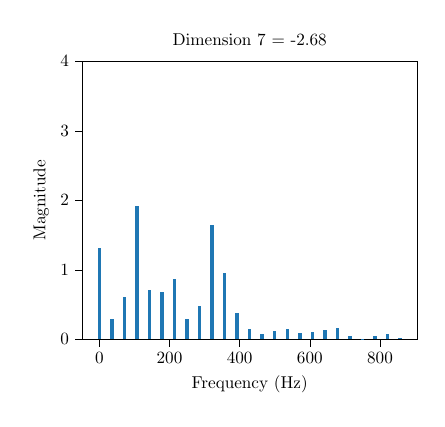
\begin{tikzpicture}[scale=0.62]

\definecolor{darkgray176}{RGB}{176,176,176}
\definecolor{steelblue31119180}{RGB}{31,119,180}

\begin{axis}[
tick align=outside,
tick pos=left,
x grid style={darkgray176},
xlabel={Frequency (Hz)},
xmin=-48.3571428571429, xmax=905.5,
xtick style={color=black},
y grid style={darkgray176},
ylabel={Magnitude},
ymin=0, ymax=4,
title={Dimension 7 = -2.68},
ytick style={color=black}
]
\draw[draw=none,fill=steelblue31119180] (axis cs:-5,0) rectangle (axis cs:5,1.31270937714726);
\draw[draw=none,fill=steelblue31119180] (axis cs:30.7142857142857,0) rectangle (axis cs:40.7142857142857,0.288125975872221);
\draw[draw=none,fill=steelblue31119180] (axis cs:66.4285714285714,0) rectangle (axis cs:76.4285714285714,0.616790952368152);
\draw[draw=none,fill=steelblue31119180] (axis cs:102.142857142857,0) rectangle (axis cs:112.142857142857,1.92312523138079);
\draw[draw=none,fill=steelblue31119180] (axis cs:137.857142857143,0) rectangle (axis cs:147.857142857143,0.707237007629874);
\draw[draw=none,fill=steelblue31119180] (axis cs:173.571428571429,0) rectangle (axis cs:183.571428571429,0.677698119881814);
\draw[draw=none,fill=steelblue31119180] (axis cs:209.285714285714,0) rectangle (axis cs:219.285714285714,0.862386040544995);
\draw[draw=none,fill=steelblue31119180] (axis cs:245,0) rectangle (axis cs:255,0.298711415685218);
\draw[draw=none,fill=steelblue31119180] (axis cs:280.714285714286,0) rectangle (axis cs:290.714285714286,0.483968708976862);
\draw[draw=none,fill=steelblue31119180] (axis cs:316.428571428571,0) rectangle (axis cs:326.428571428571,1.65269155101225);
\draw[draw=none,fill=steelblue31119180] (axis cs:352.142857142857,0) rectangle (axis cs:362.142857142857,0.951122100407993);
\draw[draw=none,fill=steelblue31119180] (axis cs:387.857142857143,0) rectangle (axis cs:397.857142857143,0.377021033569998);
\draw[draw=none,fill=steelblue31119180] (axis cs:423.571428571429,0) rectangle (axis cs:433.571428571429,0.156449857538637);
\draw[draw=none,fill=steelblue31119180] (axis cs:459.285714285714,0) rectangle (axis cs:469.285714285714,0.0846393619854383);
\draw[draw=none,fill=steelblue31119180] (axis cs:495,0) rectangle (axis cs:505,0.118818944486802);
\draw[draw=none,fill=steelblue31119180] (axis cs:530.714285714286,0) rectangle (axis cs:540.714285714286,0.143214948815801);
\draw[draw=none,fill=steelblue31119180] (axis cs:566.428571428571,0) rectangle (axis cs:576.428571428571,0.0949080699867579);
\draw[draw=none,fill=steelblue31119180] (axis cs:602.142857142857,0) rectangle (axis cs:612.142857142857,0.10757439472035);
\draw[draw=none,fill=steelblue31119180] (axis cs:637.857142857143,0) rectangle (axis cs:647.857142857143,0.131395993038413);
\draw[draw=none,fill=steelblue31119180] (axis cs:673.571428571429,0) rectangle (axis cs:683.571428571429,0.160127533802761);
\draw[draw=none,fill=steelblue31119180] (axis cs:709.285714285714,0) rectangle (axis cs:719.285714285714,0.0535699464522896);
\draw[draw=none,fill=steelblue31119180] (axis cs:745,0) rectangle (axis cs:755,0.00967304476823895);
\draw[draw=none,fill=steelblue31119180] (axis cs:780.714285714286,0) rectangle (axis cs:790.714285714286,0.0422317493349039);
\draw[draw=none,fill=steelblue31119180] (axis cs:816.428571428571,0) rectangle (axis cs:826.428571428571,0.0743497564419976);
\draw[draw=none,fill=steelblue31119180] (axis cs:852.142857142857,0) rectangle (axis cs:862.142857142857,0.0273048386393424);
\end{axis}

\end{tikzpicture}

	\end{subfigure}\hfill
	\begin{subfigure}{0.3\textwidth}
		\centering
		% This file was created with tikzplotlib v0.10.1.
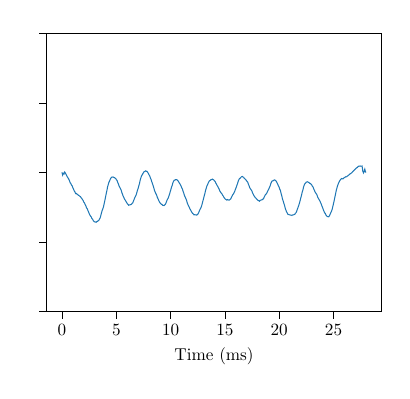
\begin{tikzpicture}[scale=0.62]

\definecolor{darkgray176}{RGB}{176,176,176}
\definecolor{steelblue31119180}{RGB}{31,119,180}

\begin{axis}[
yticklabel={\empty},
tick align=outside,
tick pos=left,
x grid style={darkgray176},
xlabel={Time (ms)},
xmin=-1.4, xmax=29.4,
xtick style={color=black},
y grid style={darkgray176},
% ylabel={Amplitude},
ymin=-0.1, ymax=0.1,
ytick style={color=black}
]
\addplot [semithick, steelblue31119180]
table {%
0 0
0.0626398210290828 -0.00193993691605009
0.125279642058166 -0.000697388132446564
0.187919463087248 -0.00111275092517369
0.250559284116331 0.00024235098553984
0.313199105145414 -0.000513447461112232
0.375838926174497 -0.00148002097020613
0.438478747203579 -0.00236590096614505
0.501118568232662 -0.00338719153914276
0.563758389261745 -0.0040478758738945
0.626398210290828 -0.00489145892378468
0.68903803131991 -0.00597273225852307
0.751677852348993 -0.0075518943669412
0.814317673378076 -0.00804388824375284
0.876957494407159 -0.00911086484564831
0.939597315436242 -0.00976522177482811
1.00223713646532 -0.0111615252149785
1.06487695749441 -0.0120892122812919
1.12751677852349 -0.0133643534484526
1.19015659955257 -0.0140450388668167
1.25279642058166 -0.0152411321678118
1.31543624161074 -0.0152015755478068
1.37807606263982 -0.0156972490801107
1.4407158836689 -0.0158916462787846
1.50335570469799 -0.0164657530043549
1.56599552572707 -0.0166319236784373
1.62863534675615 -0.0171322892138722
1.69127516778523 -0.0173743133176893
1.75391498881432 -0.0181628179505167
1.8165548098434 -0.0186722927520539
1.87919463087248 -0.0195240025227302
1.94183445190157 -0.0201793634176454
2.00447427293065 -0.0213767018969227
2.06711409395973 -0.0218668722441332
2.12975391498881 -0.0232046467170819
2.1923937360179 -0.0239699781816078
2.25503355704698 -0.0254819174265902
2.31767337807606 -0.0260842469514616
2.38031319910515 -0.02732341299021
2.44295302013423 -0.0283705943307821
2.50559284116331 -0.0296850969152363
2.56823266219239 -0.0306688831281542
2.63087248322148 -0.0315327634222355
2.69351230425056 -0.0320830301525409
2.75615212527964 -0.0332634595391534
2.81879194630872 -0.0337594674162617
2.88143176733781 -0.0346627948093134
2.94407158836689 -0.0353023716492341
3.00671140939597 -0.0356445175864352
3.06935123042506 -0.035673768940888
3.13199105145414 -0.0359154810516426
3.19463087248322 -0.035473047324375
3.2572706935123 -0.0353451175052648
3.31991051454139 -0.034851632399747
3.38255033557047 -0.0345895809540213
3.44519015659955 -0.0336693489436535
3.50782997762864 -0.0329108504115935
3.57046979865772 -0.0311585394228065
3.6331096196868 -0.0292167303671173
3.69574944071588 -0.0274955162390967
3.75838926174497 -0.0262148996452557
3.82102908277405 -0.0247058035468295
3.88366890380313 -0.0225165513962907
3.94630872483221 -0.0201710773344408
4.0089485458613 -0.0177496855815985
4.07158836689038 -0.015311727462799
4.13422818791946 -0.0130772745024238
4.19686800894855 -0.0104869296586754
4.25950782997763 -0.00871839223667079
4.32214765100671 -0.00709854418899389
4.38478747203579 -0.00616015045709858
4.44742729306488 -0.00491042862702536
4.51006711409396 -0.00406632385522927
4.57270693512304 -0.00346006396782878
4.63534675615213 -0.00342682171487968
4.69798657718121 -0.00326321851587135
4.76062639821029 -0.0036356184669089
4.82326621923937 -0.00375522114961539
4.88590604026846 -0.00417020489405466
4.94854586129754 -0.00445070286475172
5.01118568232662 -0.00530394186709551
5.0738255033557 -0.00580074416235989
5.13646532438479 -0.00734688157228216
5.19910514541387 -0.00843495169917009
5.26174496644295 -0.00992326142778933
5.32438478747204 -0.0108189789840839
5.38702460850112 -0.0118006604079832
5.4496644295302 -0.012858154283424
5.51230425055928 -0.0146084608847663
5.57494407158837 -0.0158316910629404
5.63758389261745 -0.017210534067462
5.70022371364653 -0.0182066267768809
5.76286353467562 -0.019341929859463
5.8255033557047 -0.0199633272827272
5.88814317673378 -0.0208683198805423
5.95078299776286 -0.0216582978656828
6.01342281879195 -0.022514550627878
6.07606263982103 -0.0229377234917159
6.13870246085011 -0.0236546001053296
6.2013422818792 -0.0234269479902199
6.26398210290828 -0.0233680328991789
6.32662192393736 -0.0231993186018811
6.38926174496644 -0.0230197730230405
6.45190156599553 -0.0223188432646078
6.51454138702461 -0.0219767539568195
6.57718120805369 -0.020686269068978
6.63982102908277 -0.0194335101959889
6.70246085011186 -0.0182000818543586
6.76510067114094 -0.0172540410328031
6.82774049217002 -0.016209368493983
6.89038031319911 -0.0145123920359668
6.95302013422819 -0.0128312964904928
7.01565995525727 -0.011369697843372
7.07829977628635 -0.00948762195497351
7.14093959731544 -0.00777829895358558
7.20357941834452 -0.00547778635167035
7.2662192393736 -0.00382289449815582
7.32885906040269 -0.00239693011538494
7.39149888143177 -0.001753756326417
7.45413870246085 -0.000781532301998778
7.51677852348993 6.73212836052733e-05
7.57941834451902 0.000587434764176407
7.6420581655481 0.000659656592163462
7.70469798657718 0.0011229761594894
7.76733780760626 0.000801310005704027
7.82997762863535 0.000698161930245841
7.89261744966443 -3.1259598447974e-05
7.95525727069351 -0.000749898274372888
8.0178970917226 -0.00186771298164889
8.08053691275168 -0.00256872730917179
8.14317673378076 -0.00407967935222507
8.20581655480984 -0.00523308175772228
8.26845637583893 -0.00684347297471242
8.33109619686801 -0.00807858403497094
8.39373601789709 -0.00967644710068735
8.45637583892617 -0.0112190790124388
8.51901565995526 -0.0130481103110133
8.58165548098434 -0.0142187896815922
8.64429530201342 -0.0153381289639229
8.70693512304251 -0.0162461492914281
8.76957494407159 -0.0178199395312359
8.83221476510067 -0.0188130948492545
8.89485458612975 -0.0201093304727302
8.95749440715884 -0.0210614237784339
9.02013422818792 -0.0218487176919143
9.082774049217 -0.0223928749461302
9.14541387024608 -0.0229616805836058
9.20805369127517 -0.0230043411204879
9.27069351230425 -0.0237804200475248
9.33333333333333 -0.0237110909074545
9.39597315436242 -0.0239102192248074
9.4586129753915 -0.0234278298964436
9.52125279642058 -0.0228990960941219
9.58389261744967 -0.0218231376360527
9.64653243847875 -0.0205061491703827
9.70917225950783 -0.0193424955160426
9.77181208053691 -0.018616105261065
9.834451901566 -0.0172838850146872
9.89709172259508 -0.0157916663439582
9.95973154362416 -0.0140185877930798
10.0223713646532 -0.0123708326644545
10.0850111856823 -0.0106744820552084
10.1476510067114 -0.00930849950285566
10.2102908277405 -0.00748266152812531
10.2729306487696 -0.00644440207655398
10.3355704697987 -0.00563968386776095
10.3982102908277 -0.00555548336881919
10.4608501118568 -0.00516599532991848
10.5234899328859 -0.0051542442767012
10.586129753915 -0.00529719335370816
10.6487695749441 -0.00593067748134568
10.7114093959732 -0.00634356388734691
10.7740492170022 -0.00736922608850986
10.8366890380313 -0.00803187458257147
10.8993288590604 -0.0089733005195056
10.9619686800895 -0.00978573921117807
11.0246085011186 -0.0111731671471924
11.0872483221477 -0.0119811839192806
11.1498881431767 -0.0137315380180742
11.2125279642058 -0.0149477422987455
11.2751677852349 -0.0166889945820174
11.337807606264 -0.0176660706157852
11.4004474272931 -0.0188565955391066
11.4630872483221 -0.0200510227040156
11.5257270693512 -0.0218445007633043
11.5883668903803 -0.0230041039145033
11.6510067114094 -0.0241762147278794
11.7136465324385 -0.0250530869718766
11.7762863534676 -0.0262797192714158
11.8389261744966 -0.027023786778918
11.9015659955257 -0.0280513898563265
11.9642058165548 -0.0288587481833544
12.0268456375839 -0.0295683772446925
12.089485458613 -0.0299139131960653
12.1521252796421 -0.0305846930675259
12.2147651006711 -0.0303976354407984
12.2774049217002 -0.0306569234711812
12.3400447427293 -0.0306414825179233
12.4026845637584 -0.0307158210608583
12.4653243847875 -0.0302266703306029
12.5279642058166 -0.0299377874815024
12.5906040268456 -0.0288169970173364
12.6532438478747 -0.0275692523850891
12.7158836689038 -0.0264562012115181
12.7785234899329 -0.0256634560857443
12.841163310962 -0.0244389498143788
12.9038031319911 -0.0226962687010133
12.9664429530201 -0.0207448930998377
13.0290827740492 -0.0189703644797106
13.0917225950783 -0.0169095892096626
13.1543624161074 -0.0151532614266112
13.2170022371365 -0.0129474857509536
13.2796420581655 -0.0113705251078378
13.3422818791946 -0.00967341267672561
13.4049217002237 -0.00875322164455116
13.4675615212528 -0.00757922379037478
13.5302013422819 -0.00659251304330842
13.592841163311 -0.00594735833122426
13.65548098434 -0.00570734011496873
13.7181208053691 -0.00515767018116961
13.7807606263982 -0.00519810113180804
13.8434004474273 -0.00482528749228324
13.9060402684564 -0.00515122189742807
13.9686800894855 -0.00544539820277851
14.0313199105145 -0.00606688503300984
14.0939597315436 -0.00646338295566556
14.1565995525727 -0.00763518456994687
14.2192393736018 -0.00843569395076109
14.2818791946309 -0.00947208871327391
14.34451901566 -0.0101807585123601
14.407158836689 -0.0111817509098441
14.4697986577181 -0.0120870489814638
14.5324384787472 -0.0134959457654681
14.5950782997763 -0.0141432432695323
14.6577181208054 -0.0148773754278085
14.7203579418345 -0.0154101146672596
14.7829977628635 -0.0163902547522979
14.8456375838926 -0.0170291740784809
14.9082774049217 -0.0179558711488975
14.9709172259508 -0.0186465589717131
15.0335570469799 -0.0192331361065575
15.0961968680089 -0.0195358479833043
15.158836689038 -0.0198954767078761
15.2214765100671 -0.0195587890710207
15.2841163310962 -0.0198893158277809
15.3467561521253 -0.0198336920307187
15.4093959731544 -0.019957424197721
15.4720357941834 -0.0194759885436737
15.5346756152125 -0.0190920362861564
15.5973154362416 -0.0180706887212176
15.6599552572707 -0.0169706257722722
15.7225950782998 -0.0159926750453427
15.7852348993289 -0.0154632865232509
15.8478747203579 -0.0145415439076672
15.910514541387 -0.0134155520069219
15.9731543624161 -0.0120827655164187
16.0357941834452 -0.0108127846263799
16.0984340044743 -0.00937753682018527
16.1610738255034 -0.0080538707716553
16.2237136465324 -0.00633208294892871
16.2863534675615 -0.00529039064234735
16.3489932885906 -0.00436794674086491
16.4116331096197 -0.00420468906253176
16.4742729306488 -0.0035372096170115
16.5369127516779 -0.00309298029982004
16.5995525727069 -0.00297285403256248
16.662192393736 -0.00334789148913134
16.7248322147651 -0.00356254867909339
16.7874720357942 -0.00435261607120101
16.8501118568233 -0.00472985238036853
16.9127516778523 -0.0053461461559238
16.9753914988814 -0.00567663938507138
17.0380313199105 -0.00658133582230782
17.1006711409396 -0.00707126775093927
17.1633109619687 -0.00855818980892233
17.2259507829978 -0.00963812948973387
17.2885906040268 -0.0111377743454087
17.3512304250559 -0.0117959981259184
17.413870246085 -0.0125579870737239
17.4765100671141 -0.0133017546953571
17.5391498881432 -0.0146937936094383
17.6017897091723 -0.0156262248329468
17.6644295302013 -0.0166750974553143
17.7270693512304 -0.0173641191420439
17.7897091722595 -0.0181859511532039
17.8523489932886 -0.0185211233469664
17.9149888143177 -0.0191185392139342
17.9776286353468 -0.0196192912482375
18.0402684563758 -0.0201465971517883
18.1029082774049 -0.0202752597405006
18.165548098434 -0.0207546639987486
18.2281879194631 -0.0202718090090976
18.2908277404922 -0.0199718117563917
18.3534675615213 -0.0198644418144386
18.4161073825503 -0.01982115804149
18.4787472035794 -0.0192898742779589
18.5413870246085 -0.0190784383515184
18.6040268456376 -0.0180081292961868
18.6666666666667 -0.0169898476451635
18.7293064876958 -0.0160652905727593
18.7919463087248 -0.0155984235977466
18.8545861297539 -0.0149188462719821
18.917225950783 -0.0138154529135099
18.9798657718121 -0.0127515262117822
19.0425055928412 -0.0119236599803971
19.1051454138702 -0.0107432210992947
19.1677852348993 -0.00963751154157939
19.2304250559284 -0.00792205298706989
19.2930648769575 -0.00688576142009873
19.3557046979866 -0.00610579497137126
19.4183445190157 -0.0061797442214701
19.4809843400447 -0.00575651343436849
19.5436241610738 -0.00549986924751093
19.6062639821029 -0.00550226312155691
19.668903803132 -0.00602696132189875
19.7315436241611 -0.00635458142090364
19.7941834451902 -0.00754223414540491
19.8568232662192 -0.0084792148796904
19.9194630872483 -0.00964791891508854
19.9821029082774 -0.0105099868554397
20.0447427293065 -0.0120551966680776
20.1073825503356 -0.0130137496271589
20.1700223713647 -0.0152044488717146
20.2326621923937 -0.0168635845809375
20.2953020134228 -0.019133672555721
20.3579418344519 -0.0205623124469847
20.420581655481 -0.0221308947309552
20.4832214765101 -0.0235966664532687
20.5458612975392 -0.0256366451089614
20.6085011185682 -0.0270639085054598
20.6711409395973 -0.0283343148286511
20.7337807606264 -0.0291837782492774
20.7964205816555 -0.0301544365391835
20.8590604026846 -0.0303579606990886
20.9217002237136 -0.0305262249863188
20.9843400447427 -0.0306423743249186
21.0469798657718 -0.0307146397438025
21.1096196868009 -0.0307650097689573
21.17225950783 -0.0310371947543533
21.2348993288591 -0.0305777494889378
21.2975391498881 -0.0306150344319192
21.3601789709172 -0.0303580903591926
21.4228187919463 -0.0302442793903135
21.4854586129754 -0.0294810385637035
21.5480984340045 -0.0290137161719519
21.6107382550336 -0.0278098889870332
21.6733780760626 -0.0264089604177131
21.7360178970917 -0.0250087135765176
21.7986577181208 -0.0237058942524979
21.8612975391499 -0.0220596348279275
21.923937360179 -0.02028223028369
21.9865771812081 -0.0182890103592369
22.0492170022371 -0.0164573208847702
22.1118568232662 -0.0143455547724394
22.1744966442953 -0.0127747641413804
22.2371364653244 -0.010639312633332
22.2997762863535 -0.00914210952418363
22.3624161073826 -0.00808671373723937
22.4250559284116 -0.00765494831006399
22.4876957494407 -0.00705658045016079
22.5503355704698 -0.00685571037832923
22.6129753914989 -0.00677605473355159
22.675615212528 -0.00717133541760229
22.738255033557 -0.00729907692828834
22.8008948545861 -0.00784356573334076
22.8635346756152 -0.00799461079748885
22.9261744966443 -0.00850925071402484
22.9888143176734 -0.00898205096389623
23.0514541387025 -0.00996084994442711
23.1140939597315 -0.0106121865944974
23.1767337807606 -0.0119826560777506
23.2393736017897 -0.0128798367418099
23.3020134228188 -0.01422062497461
23.3646532438479 -0.0148710731429442
23.427293064877 -0.0156335985325527
23.489932885906 -0.0165303014281312
23.5525727069351 -0.018088021696914
23.6152125279642 -0.0188820565231894
23.6778523489933 -0.0197612943265262
23.7404921700224 -0.0205219524143726
23.8031319910515 -0.0217698877864836
23.8657718120805 -0.0227528209079232
23.9284116331096 -0.024208398373335
23.9910514541387 -0.0253864640632532
24.0536912751678 -0.0268292097662319
24.1163310961969 -0.0279409261732893
24.1789709172259 -0.0291731259191796
24.241610738255 -0.0295585168888105
24.3042505592841 -0.0308126008525591
24.3668903803132 -0.031327838678188
24.4295302013423 -0.0318774218177235
24.4921700223714 -0.0318811046422128
24.5548098434004 -0.0319863388802381
24.6174496644295 -0.0312568510463774
24.6800894854586 -0.0302467762098816
24.7427293064877 -0.0290509528111691
24.8053691275168 -0.0280506531364166
24.8680089485459 -0.0266603137047699
24.9306487695749 -0.0246157685932297
24.993288590604 -0.0225176575324879
25.0559284116331 -0.0203431202786281
25.1185682326622 -0.0178945301813167
25.1812080536913 -0.0156796480335245
25.2438478747204 -0.0131607170047976
25.3064876957494 -0.0113573145908897
25.3691275167785 -0.00954080660571188
25.4317673378076 -0.0083261649030567
25.4944071588367 -0.00708915283215926
25.5570469798658 -0.00624982667649352
25.6196868008949 -0.00537700829839946
25.6823266219239 -0.00494568711209217
25.744966442953 -0.00445876410543519
25.8076062639821 -0.00463843895684953
25.8702460850112 -0.00463734595917615
25.9328859060403 -0.00417199610863756
25.9955257270694 -0.00376390583263148
26.0581655480984 -0.00351306192276862
26.1208053691275 -0.00316015437195365
26.1834451901566 -0.00319486327669365
26.2460850111857 -0.0028069100573959
26.3087248322148 -0.00251574174269734
26.3713646532438 -0.00206075192447877
26.4340044742729 -0.00175063678332223
26.496644295302 -0.00115453855653337
26.5592841163311 -0.000961863192035849
26.6219239373602 -0.000519481618832422
26.6845637583893 -0.000253477640099975
26.7472035794183 0.000386290302212607
26.8098434004474 0.000813860121189346
26.8724832214765 0.00136720877915821
26.9351230425056 0.00177161288041396
26.9977628635347 0.0023945276094163
27.0604026845638 0.0027713477986571
27.1230425055928 0.00326533768101027
27.1856823266219 0.00345150310071123
27.248322147651 0.00407087321599458
27.3109619686801 0.00446927401193436
27.3736017897092 0.00457032027360577
27.4362416107383 0.00441366212830047
27.4988814317673 0.00459057578954521
27.5615212527964 0.00445979537329818
27.6241610738255 0.00456084163496958
27.6868008948546 0.00105147996304819
27.7494407158837 -0.000385981415642188
27.8120805369128 0.00072438754891389
27.8747203579418 0.00228477716945962
27.9373601789709 0.00025185048830189
28 0
};
\end{axis}

\end{tikzpicture}

	\end{subfigure}\hfill
	\begin{subfigure}{0.3\textwidth}
		\centering
		% This file was created with tikzplotlib v0.10.1.
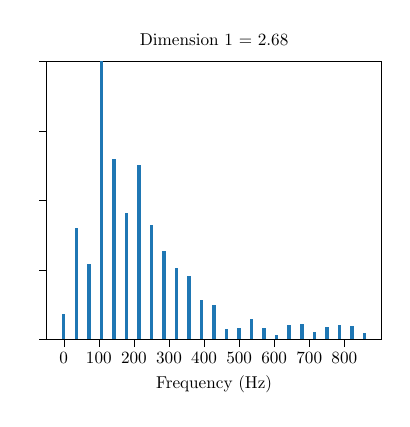
\begin{tikzpicture}[scale=0.62]

\definecolor{darkgray176}{RGB}{176,176,176}
\definecolor{steelblue31119180}{RGB}{31,119,180}

\begin{axis}[
yticklabel={\empty},
tick align=outside,
tick pos=left,
x grid style={darkgray176},
xlabel={Frequency (Hz)},
xmin=-48.3571428571429, xmax=905.5,
xtick style={color=black},
xtick={0, 100, 200, 300, 400, 500, 600, 700, 800}, % Set explicit tick positions
y grid style={darkgray176},
%ylabel={Magnitude},
ymin=0, ymax=4,
title={Dimension 1 = 2.68},
ytick style={color=black}
]
\draw[draw=none,fill=steelblue31119180] (axis cs:-5,0) rectangle (axis cs:5,0.363293109461665);
\draw[draw=none,fill=steelblue31119180] (axis cs:30.7142857142857,0) rectangle (axis cs:40.7142857142857,1.59671692845371);
\draw[draw=none,fill=steelblue31119180] (axis cs:66.4285714285714,0) rectangle (axis cs:76.4285714285714,1.08375129075336);
\draw[draw=none,fill=steelblue31119180] (axis cs:102.142857142857,0) rectangle (axis cs:112.142857142857,5.72028640718505);
\draw[draw=none,fill=steelblue31119180] (axis cs:137.857142857143,0) rectangle (axis cs:147.857142857143,2.60109171070077);
\draw[draw=none,fill=steelblue31119180] (axis cs:173.571428571429,0) rectangle (axis cs:183.571428571429,1.82230187959835);
\draw[draw=none,fill=steelblue31119180] (axis cs:209.285714285714,0) rectangle (axis cs:219.285714285714,2.50466396839656);
\draw[draw=none,fill=steelblue31119180] (axis cs:245,0) rectangle (axis cs:255,1.64154431128106);
\draw[draw=none,fill=steelblue31119180] (axis cs:280.714285714286,0) rectangle (axis cs:290.714285714286,1.2779936763853);
\draw[draw=none,fill=steelblue31119180] (axis cs:316.428571428571,0) rectangle (axis cs:326.428571428571,1.02566988726104);
\draw[draw=none,fill=steelblue31119180] (axis cs:352.142857142857,0) rectangle (axis cs:362.142857142857,0.906444113984638);
\draw[draw=none,fill=steelblue31119180] (axis cs:387.857142857143,0) rectangle (axis cs:397.857142857143,0.567573738688084);
\draw[draw=none,fill=steelblue31119180] (axis cs:423.571428571429,0) rectangle (axis cs:433.571428571429,0.497884322563813);
\draw[draw=none,fill=steelblue31119180] (axis cs:459.285714285714,0) rectangle (axis cs:469.285714285714,0.143370970638671);
\draw[draw=none,fill=steelblue31119180] (axis cs:495,0) rectangle (axis cs:505,0.158030205491621);
\draw[draw=none,fill=steelblue31119180] (axis cs:530.714285714286,0) rectangle (axis cs:540.714285714286,0.287791882784369);
\draw[draw=none,fill=steelblue31119180] (axis cs:566.428571428571,0) rectangle (axis cs:576.428571428571,0.164560600100172);
\draw[draw=none,fill=steelblue31119180] (axis cs:602.142857142857,0) rectangle (axis cs:612.142857142857,0.0653538748355305);
\draw[draw=none,fill=steelblue31119180] (axis cs:637.857142857143,0) rectangle (axis cs:647.857142857143,0.209706204538538);
\draw[draw=none,fill=steelblue31119180] (axis cs:673.571428571429,0) rectangle (axis cs:683.571428571429,0.216581742305538);
\draw[draw=none,fill=steelblue31119180] (axis cs:709.285714285714,0) rectangle (axis cs:719.285714285714,0.104565114650486);
\draw[draw=none,fill=steelblue31119180] (axis cs:745,0) rectangle (axis cs:755,0.18370350932939);
\draw[draw=none,fill=steelblue31119180] (axis cs:780.714285714286,0) rectangle (axis cs:790.714285714286,0.206670350113575);
\draw[draw=none,fill=steelblue31119180] (axis cs:816.428571428571,0) rectangle (axis cs:826.428571428571,0.196489132073225);
\draw[draw=none,fill=steelblue31119180] (axis cs:852.142857142857,0) rectangle (axis cs:862.142857142857,0.0885177801919891);
\end{axis}

\end{tikzpicture}

	\end{subfigure}
	
	\vspace{0.5cm} % Adjust vertical spacing between rows
	
	\begin{subfigure}{0.36\textwidth}
		\centering
		% This file was created with tikzplotlib v0.10.1.
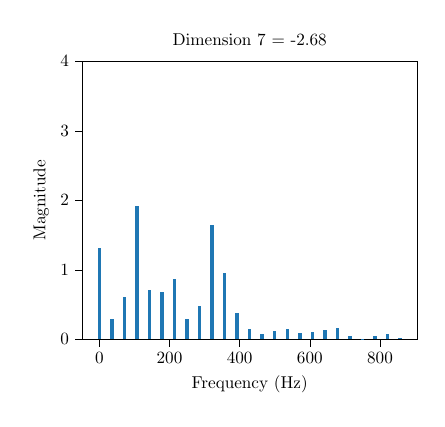
\begin{tikzpicture}[scale=0.62]

\definecolor{darkgray176}{RGB}{176,176,176}
\definecolor{steelblue31119180}{RGB}{31,119,180}

\begin{axis}[
tick align=outside,
tick pos=left,
x grid style={darkgray176},
xlabel={Frequency (Hz)},
xmin=-48.3571428571429, xmax=905.5,
xtick style={color=black},
y grid style={darkgray176},
ylabel={Magnitude},
ymin=0, ymax=4,
title={Dimension 7 = -2.68},
ytick style={color=black}
]
\draw[draw=none,fill=steelblue31119180] (axis cs:-5,0) rectangle (axis cs:5,1.31270937714726);
\draw[draw=none,fill=steelblue31119180] (axis cs:30.7142857142857,0) rectangle (axis cs:40.7142857142857,0.288125975872221);
\draw[draw=none,fill=steelblue31119180] (axis cs:66.4285714285714,0) rectangle (axis cs:76.4285714285714,0.616790952368152);
\draw[draw=none,fill=steelblue31119180] (axis cs:102.142857142857,0) rectangle (axis cs:112.142857142857,1.92312523138079);
\draw[draw=none,fill=steelblue31119180] (axis cs:137.857142857143,0) rectangle (axis cs:147.857142857143,0.707237007629874);
\draw[draw=none,fill=steelblue31119180] (axis cs:173.571428571429,0) rectangle (axis cs:183.571428571429,0.677698119881814);
\draw[draw=none,fill=steelblue31119180] (axis cs:209.285714285714,0) rectangle (axis cs:219.285714285714,0.862386040544995);
\draw[draw=none,fill=steelblue31119180] (axis cs:245,0) rectangle (axis cs:255,0.298711415685218);
\draw[draw=none,fill=steelblue31119180] (axis cs:280.714285714286,0) rectangle (axis cs:290.714285714286,0.483968708976862);
\draw[draw=none,fill=steelblue31119180] (axis cs:316.428571428571,0) rectangle (axis cs:326.428571428571,1.65269155101225);
\draw[draw=none,fill=steelblue31119180] (axis cs:352.142857142857,0) rectangle (axis cs:362.142857142857,0.951122100407993);
\draw[draw=none,fill=steelblue31119180] (axis cs:387.857142857143,0) rectangle (axis cs:397.857142857143,0.377021033569998);
\draw[draw=none,fill=steelblue31119180] (axis cs:423.571428571429,0) rectangle (axis cs:433.571428571429,0.156449857538637);
\draw[draw=none,fill=steelblue31119180] (axis cs:459.285714285714,0) rectangle (axis cs:469.285714285714,0.0846393619854383);
\draw[draw=none,fill=steelblue31119180] (axis cs:495,0) rectangle (axis cs:505,0.118818944486802);
\draw[draw=none,fill=steelblue31119180] (axis cs:530.714285714286,0) rectangle (axis cs:540.714285714286,0.143214948815801);
\draw[draw=none,fill=steelblue31119180] (axis cs:566.428571428571,0) rectangle (axis cs:576.428571428571,0.0949080699867579);
\draw[draw=none,fill=steelblue31119180] (axis cs:602.142857142857,0) rectangle (axis cs:612.142857142857,0.10757439472035);
\draw[draw=none,fill=steelblue31119180] (axis cs:637.857142857143,0) rectangle (axis cs:647.857142857143,0.131395993038413);
\draw[draw=none,fill=steelblue31119180] (axis cs:673.571428571429,0) rectangle (axis cs:683.571428571429,0.160127533802761);
\draw[draw=none,fill=steelblue31119180] (axis cs:709.285714285714,0) rectangle (axis cs:719.285714285714,0.0535699464522896);
\draw[draw=none,fill=steelblue31119180] (axis cs:745,0) rectangle (axis cs:755,0.00967304476823895);
\draw[draw=none,fill=steelblue31119180] (axis cs:780.714285714286,0) rectangle (axis cs:790.714285714286,0.0422317493349039);
\draw[draw=none,fill=steelblue31119180] (axis cs:816.428571428571,0) rectangle (axis cs:826.428571428571,0.0743497564419976);
\draw[draw=none,fill=steelblue31119180] (axis cs:852.142857142857,0) rectangle (axis cs:862.142857142857,0.0273048386393424);
\end{axis}

\end{tikzpicture}

	\end{subfigure}\hfill
	\begin{subfigure}{0.3\textwidth}
		\centering
		% This file was created with tikzplotlib v0.10.1.
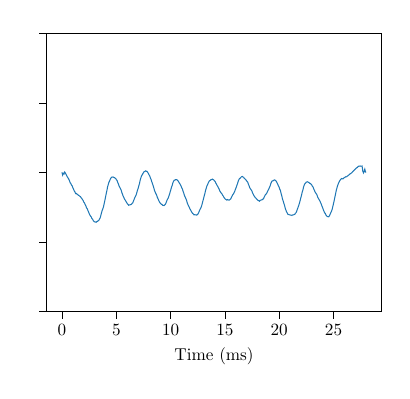
\begin{tikzpicture}[scale=0.62]

\definecolor{darkgray176}{RGB}{176,176,176}
\definecolor{steelblue31119180}{RGB}{31,119,180}

\begin{axis}[
yticklabel={\empty},
tick align=outside,
tick pos=left,
x grid style={darkgray176},
xlabel={Time (ms)},
xmin=-1.4, xmax=29.4,
xtick style={color=black},
y grid style={darkgray176},
% ylabel={Amplitude},
ymin=-0.1, ymax=0.1,
ytick style={color=black}
]
\addplot [semithick, steelblue31119180]
table {%
0 0
0.0626398210290828 -0.00193993691605009
0.125279642058166 -0.000697388132446564
0.187919463087248 -0.00111275092517369
0.250559284116331 0.00024235098553984
0.313199105145414 -0.000513447461112232
0.375838926174497 -0.00148002097020613
0.438478747203579 -0.00236590096614505
0.501118568232662 -0.00338719153914276
0.563758389261745 -0.0040478758738945
0.626398210290828 -0.00489145892378468
0.68903803131991 -0.00597273225852307
0.751677852348993 -0.0075518943669412
0.814317673378076 -0.00804388824375284
0.876957494407159 -0.00911086484564831
0.939597315436242 -0.00976522177482811
1.00223713646532 -0.0111615252149785
1.06487695749441 -0.0120892122812919
1.12751677852349 -0.0133643534484526
1.19015659955257 -0.0140450388668167
1.25279642058166 -0.0152411321678118
1.31543624161074 -0.0152015755478068
1.37807606263982 -0.0156972490801107
1.4407158836689 -0.0158916462787846
1.50335570469799 -0.0164657530043549
1.56599552572707 -0.0166319236784373
1.62863534675615 -0.0171322892138722
1.69127516778523 -0.0173743133176893
1.75391498881432 -0.0181628179505167
1.8165548098434 -0.0186722927520539
1.87919463087248 -0.0195240025227302
1.94183445190157 -0.0201793634176454
2.00447427293065 -0.0213767018969227
2.06711409395973 -0.0218668722441332
2.12975391498881 -0.0232046467170819
2.1923937360179 -0.0239699781816078
2.25503355704698 -0.0254819174265902
2.31767337807606 -0.0260842469514616
2.38031319910515 -0.02732341299021
2.44295302013423 -0.0283705943307821
2.50559284116331 -0.0296850969152363
2.56823266219239 -0.0306688831281542
2.63087248322148 -0.0315327634222355
2.69351230425056 -0.0320830301525409
2.75615212527964 -0.0332634595391534
2.81879194630872 -0.0337594674162617
2.88143176733781 -0.0346627948093134
2.94407158836689 -0.0353023716492341
3.00671140939597 -0.0356445175864352
3.06935123042506 -0.035673768940888
3.13199105145414 -0.0359154810516426
3.19463087248322 -0.035473047324375
3.2572706935123 -0.0353451175052648
3.31991051454139 -0.034851632399747
3.38255033557047 -0.0345895809540213
3.44519015659955 -0.0336693489436535
3.50782997762864 -0.0329108504115935
3.57046979865772 -0.0311585394228065
3.6331096196868 -0.0292167303671173
3.69574944071588 -0.0274955162390967
3.75838926174497 -0.0262148996452557
3.82102908277405 -0.0247058035468295
3.88366890380313 -0.0225165513962907
3.94630872483221 -0.0201710773344408
4.0089485458613 -0.0177496855815985
4.07158836689038 -0.015311727462799
4.13422818791946 -0.0130772745024238
4.19686800894855 -0.0104869296586754
4.25950782997763 -0.00871839223667079
4.32214765100671 -0.00709854418899389
4.38478747203579 -0.00616015045709858
4.44742729306488 -0.00491042862702536
4.51006711409396 -0.00406632385522927
4.57270693512304 -0.00346006396782878
4.63534675615213 -0.00342682171487968
4.69798657718121 -0.00326321851587135
4.76062639821029 -0.0036356184669089
4.82326621923937 -0.00375522114961539
4.88590604026846 -0.00417020489405466
4.94854586129754 -0.00445070286475172
5.01118568232662 -0.00530394186709551
5.0738255033557 -0.00580074416235989
5.13646532438479 -0.00734688157228216
5.19910514541387 -0.00843495169917009
5.26174496644295 -0.00992326142778933
5.32438478747204 -0.0108189789840839
5.38702460850112 -0.0118006604079832
5.4496644295302 -0.012858154283424
5.51230425055928 -0.0146084608847663
5.57494407158837 -0.0158316910629404
5.63758389261745 -0.017210534067462
5.70022371364653 -0.0182066267768809
5.76286353467562 -0.019341929859463
5.8255033557047 -0.0199633272827272
5.88814317673378 -0.0208683198805423
5.95078299776286 -0.0216582978656828
6.01342281879195 -0.022514550627878
6.07606263982103 -0.0229377234917159
6.13870246085011 -0.0236546001053296
6.2013422818792 -0.0234269479902199
6.26398210290828 -0.0233680328991789
6.32662192393736 -0.0231993186018811
6.38926174496644 -0.0230197730230405
6.45190156599553 -0.0223188432646078
6.51454138702461 -0.0219767539568195
6.57718120805369 -0.020686269068978
6.63982102908277 -0.0194335101959889
6.70246085011186 -0.0182000818543586
6.76510067114094 -0.0172540410328031
6.82774049217002 -0.016209368493983
6.89038031319911 -0.0145123920359668
6.95302013422819 -0.0128312964904928
7.01565995525727 -0.011369697843372
7.07829977628635 -0.00948762195497351
7.14093959731544 -0.00777829895358558
7.20357941834452 -0.00547778635167035
7.2662192393736 -0.00382289449815582
7.32885906040269 -0.00239693011538494
7.39149888143177 -0.001753756326417
7.45413870246085 -0.000781532301998778
7.51677852348993 6.73212836052733e-05
7.57941834451902 0.000587434764176407
7.6420581655481 0.000659656592163462
7.70469798657718 0.0011229761594894
7.76733780760626 0.000801310005704027
7.82997762863535 0.000698161930245841
7.89261744966443 -3.1259598447974e-05
7.95525727069351 -0.000749898274372888
8.0178970917226 -0.00186771298164889
8.08053691275168 -0.00256872730917179
8.14317673378076 -0.00407967935222507
8.20581655480984 -0.00523308175772228
8.26845637583893 -0.00684347297471242
8.33109619686801 -0.00807858403497094
8.39373601789709 -0.00967644710068735
8.45637583892617 -0.0112190790124388
8.51901565995526 -0.0130481103110133
8.58165548098434 -0.0142187896815922
8.64429530201342 -0.0153381289639229
8.70693512304251 -0.0162461492914281
8.76957494407159 -0.0178199395312359
8.83221476510067 -0.0188130948492545
8.89485458612975 -0.0201093304727302
8.95749440715884 -0.0210614237784339
9.02013422818792 -0.0218487176919143
9.082774049217 -0.0223928749461302
9.14541387024608 -0.0229616805836058
9.20805369127517 -0.0230043411204879
9.27069351230425 -0.0237804200475248
9.33333333333333 -0.0237110909074545
9.39597315436242 -0.0239102192248074
9.4586129753915 -0.0234278298964436
9.52125279642058 -0.0228990960941219
9.58389261744967 -0.0218231376360527
9.64653243847875 -0.0205061491703827
9.70917225950783 -0.0193424955160426
9.77181208053691 -0.018616105261065
9.834451901566 -0.0172838850146872
9.89709172259508 -0.0157916663439582
9.95973154362416 -0.0140185877930798
10.0223713646532 -0.0123708326644545
10.0850111856823 -0.0106744820552084
10.1476510067114 -0.00930849950285566
10.2102908277405 -0.00748266152812531
10.2729306487696 -0.00644440207655398
10.3355704697987 -0.00563968386776095
10.3982102908277 -0.00555548336881919
10.4608501118568 -0.00516599532991848
10.5234899328859 -0.0051542442767012
10.586129753915 -0.00529719335370816
10.6487695749441 -0.00593067748134568
10.7114093959732 -0.00634356388734691
10.7740492170022 -0.00736922608850986
10.8366890380313 -0.00803187458257147
10.8993288590604 -0.0089733005195056
10.9619686800895 -0.00978573921117807
11.0246085011186 -0.0111731671471924
11.0872483221477 -0.0119811839192806
11.1498881431767 -0.0137315380180742
11.2125279642058 -0.0149477422987455
11.2751677852349 -0.0166889945820174
11.337807606264 -0.0176660706157852
11.4004474272931 -0.0188565955391066
11.4630872483221 -0.0200510227040156
11.5257270693512 -0.0218445007633043
11.5883668903803 -0.0230041039145033
11.6510067114094 -0.0241762147278794
11.7136465324385 -0.0250530869718766
11.7762863534676 -0.0262797192714158
11.8389261744966 -0.027023786778918
11.9015659955257 -0.0280513898563265
11.9642058165548 -0.0288587481833544
12.0268456375839 -0.0295683772446925
12.089485458613 -0.0299139131960653
12.1521252796421 -0.0305846930675259
12.2147651006711 -0.0303976354407984
12.2774049217002 -0.0306569234711812
12.3400447427293 -0.0306414825179233
12.4026845637584 -0.0307158210608583
12.4653243847875 -0.0302266703306029
12.5279642058166 -0.0299377874815024
12.5906040268456 -0.0288169970173364
12.6532438478747 -0.0275692523850891
12.7158836689038 -0.0264562012115181
12.7785234899329 -0.0256634560857443
12.841163310962 -0.0244389498143788
12.9038031319911 -0.0226962687010133
12.9664429530201 -0.0207448930998377
13.0290827740492 -0.0189703644797106
13.0917225950783 -0.0169095892096626
13.1543624161074 -0.0151532614266112
13.2170022371365 -0.0129474857509536
13.2796420581655 -0.0113705251078378
13.3422818791946 -0.00967341267672561
13.4049217002237 -0.00875322164455116
13.4675615212528 -0.00757922379037478
13.5302013422819 -0.00659251304330842
13.592841163311 -0.00594735833122426
13.65548098434 -0.00570734011496873
13.7181208053691 -0.00515767018116961
13.7807606263982 -0.00519810113180804
13.8434004474273 -0.00482528749228324
13.9060402684564 -0.00515122189742807
13.9686800894855 -0.00544539820277851
14.0313199105145 -0.00606688503300984
14.0939597315436 -0.00646338295566556
14.1565995525727 -0.00763518456994687
14.2192393736018 -0.00843569395076109
14.2818791946309 -0.00947208871327391
14.34451901566 -0.0101807585123601
14.407158836689 -0.0111817509098441
14.4697986577181 -0.0120870489814638
14.5324384787472 -0.0134959457654681
14.5950782997763 -0.0141432432695323
14.6577181208054 -0.0148773754278085
14.7203579418345 -0.0154101146672596
14.7829977628635 -0.0163902547522979
14.8456375838926 -0.0170291740784809
14.9082774049217 -0.0179558711488975
14.9709172259508 -0.0186465589717131
15.0335570469799 -0.0192331361065575
15.0961968680089 -0.0195358479833043
15.158836689038 -0.0198954767078761
15.2214765100671 -0.0195587890710207
15.2841163310962 -0.0198893158277809
15.3467561521253 -0.0198336920307187
15.4093959731544 -0.019957424197721
15.4720357941834 -0.0194759885436737
15.5346756152125 -0.0190920362861564
15.5973154362416 -0.0180706887212176
15.6599552572707 -0.0169706257722722
15.7225950782998 -0.0159926750453427
15.7852348993289 -0.0154632865232509
15.8478747203579 -0.0145415439076672
15.910514541387 -0.0134155520069219
15.9731543624161 -0.0120827655164187
16.0357941834452 -0.0108127846263799
16.0984340044743 -0.00937753682018527
16.1610738255034 -0.0080538707716553
16.2237136465324 -0.00633208294892871
16.2863534675615 -0.00529039064234735
16.3489932885906 -0.00436794674086491
16.4116331096197 -0.00420468906253176
16.4742729306488 -0.0035372096170115
16.5369127516779 -0.00309298029982004
16.5995525727069 -0.00297285403256248
16.662192393736 -0.00334789148913134
16.7248322147651 -0.00356254867909339
16.7874720357942 -0.00435261607120101
16.8501118568233 -0.00472985238036853
16.9127516778523 -0.0053461461559238
16.9753914988814 -0.00567663938507138
17.0380313199105 -0.00658133582230782
17.1006711409396 -0.00707126775093927
17.1633109619687 -0.00855818980892233
17.2259507829978 -0.00963812948973387
17.2885906040268 -0.0111377743454087
17.3512304250559 -0.0117959981259184
17.413870246085 -0.0125579870737239
17.4765100671141 -0.0133017546953571
17.5391498881432 -0.0146937936094383
17.6017897091723 -0.0156262248329468
17.6644295302013 -0.0166750974553143
17.7270693512304 -0.0173641191420439
17.7897091722595 -0.0181859511532039
17.8523489932886 -0.0185211233469664
17.9149888143177 -0.0191185392139342
17.9776286353468 -0.0196192912482375
18.0402684563758 -0.0201465971517883
18.1029082774049 -0.0202752597405006
18.165548098434 -0.0207546639987486
18.2281879194631 -0.0202718090090976
18.2908277404922 -0.0199718117563917
18.3534675615213 -0.0198644418144386
18.4161073825503 -0.01982115804149
18.4787472035794 -0.0192898742779589
18.5413870246085 -0.0190784383515184
18.6040268456376 -0.0180081292961868
18.6666666666667 -0.0169898476451635
18.7293064876958 -0.0160652905727593
18.7919463087248 -0.0155984235977466
18.8545861297539 -0.0149188462719821
18.917225950783 -0.0138154529135099
18.9798657718121 -0.0127515262117822
19.0425055928412 -0.0119236599803971
19.1051454138702 -0.0107432210992947
19.1677852348993 -0.00963751154157939
19.2304250559284 -0.00792205298706989
19.2930648769575 -0.00688576142009873
19.3557046979866 -0.00610579497137126
19.4183445190157 -0.0061797442214701
19.4809843400447 -0.00575651343436849
19.5436241610738 -0.00549986924751093
19.6062639821029 -0.00550226312155691
19.668903803132 -0.00602696132189875
19.7315436241611 -0.00635458142090364
19.7941834451902 -0.00754223414540491
19.8568232662192 -0.0084792148796904
19.9194630872483 -0.00964791891508854
19.9821029082774 -0.0105099868554397
20.0447427293065 -0.0120551966680776
20.1073825503356 -0.0130137496271589
20.1700223713647 -0.0152044488717146
20.2326621923937 -0.0168635845809375
20.2953020134228 -0.019133672555721
20.3579418344519 -0.0205623124469847
20.420581655481 -0.0221308947309552
20.4832214765101 -0.0235966664532687
20.5458612975392 -0.0256366451089614
20.6085011185682 -0.0270639085054598
20.6711409395973 -0.0283343148286511
20.7337807606264 -0.0291837782492774
20.7964205816555 -0.0301544365391835
20.8590604026846 -0.0303579606990886
20.9217002237136 -0.0305262249863188
20.9843400447427 -0.0306423743249186
21.0469798657718 -0.0307146397438025
21.1096196868009 -0.0307650097689573
21.17225950783 -0.0310371947543533
21.2348993288591 -0.0305777494889378
21.2975391498881 -0.0306150344319192
21.3601789709172 -0.0303580903591926
21.4228187919463 -0.0302442793903135
21.4854586129754 -0.0294810385637035
21.5480984340045 -0.0290137161719519
21.6107382550336 -0.0278098889870332
21.6733780760626 -0.0264089604177131
21.7360178970917 -0.0250087135765176
21.7986577181208 -0.0237058942524979
21.8612975391499 -0.0220596348279275
21.923937360179 -0.02028223028369
21.9865771812081 -0.0182890103592369
22.0492170022371 -0.0164573208847702
22.1118568232662 -0.0143455547724394
22.1744966442953 -0.0127747641413804
22.2371364653244 -0.010639312633332
22.2997762863535 -0.00914210952418363
22.3624161073826 -0.00808671373723937
22.4250559284116 -0.00765494831006399
22.4876957494407 -0.00705658045016079
22.5503355704698 -0.00685571037832923
22.6129753914989 -0.00677605473355159
22.675615212528 -0.00717133541760229
22.738255033557 -0.00729907692828834
22.8008948545861 -0.00784356573334076
22.8635346756152 -0.00799461079748885
22.9261744966443 -0.00850925071402484
22.9888143176734 -0.00898205096389623
23.0514541387025 -0.00996084994442711
23.1140939597315 -0.0106121865944974
23.1767337807606 -0.0119826560777506
23.2393736017897 -0.0128798367418099
23.3020134228188 -0.01422062497461
23.3646532438479 -0.0148710731429442
23.427293064877 -0.0156335985325527
23.489932885906 -0.0165303014281312
23.5525727069351 -0.018088021696914
23.6152125279642 -0.0188820565231894
23.6778523489933 -0.0197612943265262
23.7404921700224 -0.0205219524143726
23.8031319910515 -0.0217698877864836
23.8657718120805 -0.0227528209079232
23.9284116331096 -0.024208398373335
23.9910514541387 -0.0253864640632532
24.0536912751678 -0.0268292097662319
24.1163310961969 -0.0279409261732893
24.1789709172259 -0.0291731259191796
24.241610738255 -0.0295585168888105
24.3042505592841 -0.0308126008525591
24.3668903803132 -0.031327838678188
24.4295302013423 -0.0318774218177235
24.4921700223714 -0.0318811046422128
24.5548098434004 -0.0319863388802381
24.6174496644295 -0.0312568510463774
24.6800894854586 -0.0302467762098816
24.7427293064877 -0.0290509528111691
24.8053691275168 -0.0280506531364166
24.8680089485459 -0.0266603137047699
24.9306487695749 -0.0246157685932297
24.993288590604 -0.0225176575324879
25.0559284116331 -0.0203431202786281
25.1185682326622 -0.0178945301813167
25.1812080536913 -0.0156796480335245
25.2438478747204 -0.0131607170047976
25.3064876957494 -0.0113573145908897
25.3691275167785 -0.00954080660571188
25.4317673378076 -0.0083261649030567
25.4944071588367 -0.00708915283215926
25.5570469798658 -0.00624982667649352
25.6196868008949 -0.00537700829839946
25.6823266219239 -0.00494568711209217
25.744966442953 -0.00445876410543519
25.8076062639821 -0.00463843895684953
25.8702460850112 -0.00463734595917615
25.9328859060403 -0.00417199610863756
25.9955257270694 -0.00376390583263148
26.0581655480984 -0.00351306192276862
26.1208053691275 -0.00316015437195365
26.1834451901566 -0.00319486327669365
26.2460850111857 -0.0028069100573959
26.3087248322148 -0.00251574174269734
26.3713646532438 -0.00206075192447877
26.4340044742729 -0.00175063678332223
26.496644295302 -0.00115453855653337
26.5592841163311 -0.000961863192035849
26.6219239373602 -0.000519481618832422
26.6845637583893 -0.000253477640099975
26.7472035794183 0.000386290302212607
26.8098434004474 0.000813860121189346
26.8724832214765 0.00136720877915821
26.9351230425056 0.00177161288041396
26.9977628635347 0.0023945276094163
27.0604026845638 0.0027713477986571
27.1230425055928 0.00326533768101027
27.1856823266219 0.00345150310071123
27.248322147651 0.00407087321599458
27.3109619686801 0.00446927401193436
27.3736017897092 0.00457032027360577
27.4362416107383 0.00441366212830047
27.4988814317673 0.00459057578954521
27.5615212527964 0.00445979537329818
27.6241610738255 0.00456084163496958
27.6868008948546 0.00105147996304819
27.7494407158837 -0.000385981415642188
27.8120805369128 0.00072438754891389
27.8747203579418 0.00228477716945962
27.9373601789709 0.00025185048830189
28 0
};
\end{axis}

\end{tikzpicture}

	\end{subfigure}\hfill
	\begin{subfigure}{0.3\textwidth}
		\centering
		% This file was created with tikzplotlib v0.10.1.
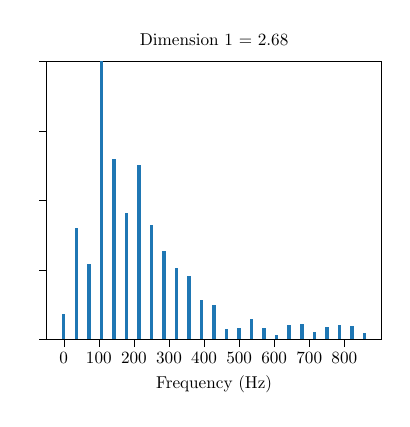
\begin{tikzpicture}[scale=0.62]

\definecolor{darkgray176}{RGB}{176,176,176}
\definecolor{steelblue31119180}{RGB}{31,119,180}

\begin{axis}[
yticklabel={\empty},
tick align=outside,
tick pos=left,
x grid style={darkgray176},
xlabel={Frequency (Hz)},
xmin=-48.3571428571429, xmax=905.5,
xtick style={color=black},
xtick={0, 100, 200, 300, 400, 500, 600, 700, 800}, % Set explicit tick positions
y grid style={darkgray176},
%ylabel={Magnitude},
ymin=0, ymax=4,
title={Dimension 1 = 2.68},
ytick style={color=black}
]
\draw[draw=none,fill=steelblue31119180] (axis cs:-5,0) rectangle (axis cs:5,0.363293109461665);
\draw[draw=none,fill=steelblue31119180] (axis cs:30.7142857142857,0) rectangle (axis cs:40.7142857142857,1.59671692845371);
\draw[draw=none,fill=steelblue31119180] (axis cs:66.4285714285714,0) rectangle (axis cs:76.4285714285714,1.08375129075336);
\draw[draw=none,fill=steelblue31119180] (axis cs:102.142857142857,0) rectangle (axis cs:112.142857142857,5.72028640718505);
\draw[draw=none,fill=steelblue31119180] (axis cs:137.857142857143,0) rectangle (axis cs:147.857142857143,2.60109171070077);
\draw[draw=none,fill=steelblue31119180] (axis cs:173.571428571429,0) rectangle (axis cs:183.571428571429,1.82230187959835);
\draw[draw=none,fill=steelblue31119180] (axis cs:209.285714285714,0) rectangle (axis cs:219.285714285714,2.50466396839656);
\draw[draw=none,fill=steelblue31119180] (axis cs:245,0) rectangle (axis cs:255,1.64154431128106);
\draw[draw=none,fill=steelblue31119180] (axis cs:280.714285714286,0) rectangle (axis cs:290.714285714286,1.2779936763853);
\draw[draw=none,fill=steelblue31119180] (axis cs:316.428571428571,0) rectangle (axis cs:326.428571428571,1.02566988726104);
\draw[draw=none,fill=steelblue31119180] (axis cs:352.142857142857,0) rectangle (axis cs:362.142857142857,0.906444113984638);
\draw[draw=none,fill=steelblue31119180] (axis cs:387.857142857143,0) rectangle (axis cs:397.857142857143,0.567573738688084);
\draw[draw=none,fill=steelblue31119180] (axis cs:423.571428571429,0) rectangle (axis cs:433.571428571429,0.497884322563813);
\draw[draw=none,fill=steelblue31119180] (axis cs:459.285714285714,0) rectangle (axis cs:469.285714285714,0.143370970638671);
\draw[draw=none,fill=steelblue31119180] (axis cs:495,0) rectangle (axis cs:505,0.158030205491621);
\draw[draw=none,fill=steelblue31119180] (axis cs:530.714285714286,0) rectangle (axis cs:540.714285714286,0.287791882784369);
\draw[draw=none,fill=steelblue31119180] (axis cs:566.428571428571,0) rectangle (axis cs:576.428571428571,0.164560600100172);
\draw[draw=none,fill=steelblue31119180] (axis cs:602.142857142857,0) rectangle (axis cs:612.142857142857,0.0653538748355305);
\draw[draw=none,fill=steelblue31119180] (axis cs:637.857142857143,0) rectangle (axis cs:647.857142857143,0.209706204538538);
\draw[draw=none,fill=steelblue31119180] (axis cs:673.571428571429,0) rectangle (axis cs:683.571428571429,0.216581742305538);
\draw[draw=none,fill=steelblue31119180] (axis cs:709.285714285714,0) rectangle (axis cs:719.285714285714,0.104565114650486);
\draw[draw=none,fill=steelblue31119180] (axis cs:745,0) rectangle (axis cs:755,0.18370350932939);
\draw[draw=none,fill=steelblue31119180] (axis cs:780.714285714286,0) rectangle (axis cs:790.714285714286,0.206670350113575);
\draw[draw=none,fill=steelblue31119180] (axis cs:816.428571428571,0) rectangle (axis cs:826.428571428571,0.196489132073225);
\draw[draw=none,fill=steelblue31119180] (axis cs:852.142857142857,0) rectangle (axis cs:862.142857142857,0.0885177801919891);
\end{axis}

\end{tikzpicture}

	\end{subfigure}
	
	\caption{The seventh dimension is being modified, while other dimensions are fixed at 0. We observe no significant differences when adjusting, indicating that the dimension may not capture any information at all.}
	\label{fig:interpol_dim7}
\end{figure}


% one dimension
\begin{figure}
	\centering
	\begin{subfigure}{0.34\textwidth}
		\centering
		% This file was created with tikzplotlib v0.10.1.
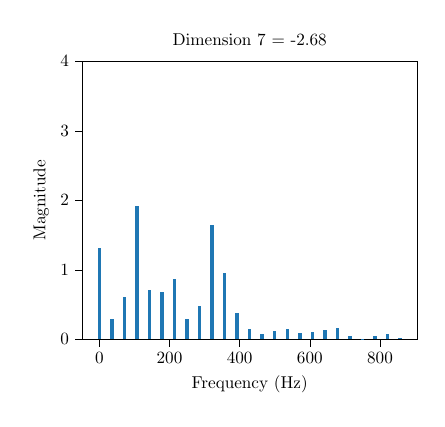
\begin{tikzpicture}[scale=0.62]

\definecolor{darkgray176}{RGB}{176,176,176}
\definecolor{steelblue31119180}{RGB}{31,119,180}

\begin{axis}[
tick align=outside,
tick pos=left,
x grid style={darkgray176},
xlabel={Frequency (Hz)},
xmin=-48.3571428571429, xmax=905.5,
xtick style={color=black},
y grid style={darkgray176},
ylabel={Magnitude},
ymin=0, ymax=4,
title={Dimension 7 = -2.68},
ytick style={color=black}
]
\draw[draw=none,fill=steelblue31119180] (axis cs:-5,0) rectangle (axis cs:5,1.31270937714726);
\draw[draw=none,fill=steelblue31119180] (axis cs:30.7142857142857,0) rectangle (axis cs:40.7142857142857,0.288125975872221);
\draw[draw=none,fill=steelblue31119180] (axis cs:66.4285714285714,0) rectangle (axis cs:76.4285714285714,0.616790952368152);
\draw[draw=none,fill=steelblue31119180] (axis cs:102.142857142857,0) rectangle (axis cs:112.142857142857,1.92312523138079);
\draw[draw=none,fill=steelblue31119180] (axis cs:137.857142857143,0) rectangle (axis cs:147.857142857143,0.707237007629874);
\draw[draw=none,fill=steelblue31119180] (axis cs:173.571428571429,0) rectangle (axis cs:183.571428571429,0.677698119881814);
\draw[draw=none,fill=steelblue31119180] (axis cs:209.285714285714,0) rectangle (axis cs:219.285714285714,0.862386040544995);
\draw[draw=none,fill=steelblue31119180] (axis cs:245,0) rectangle (axis cs:255,0.298711415685218);
\draw[draw=none,fill=steelblue31119180] (axis cs:280.714285714286,0) rectangle (axis cs:290.714285714286,0.483968708976862);
\draw[draw=none,fill=steelblue31119180] (axis cs:316.428571428571,0) rectangle (axis cs:326.428571428571,1.65269155101225);
\draw[draw=none,fill=steelblue31119180] (axis cs:352.142857142857,0) rectangle (axis cs:362.142857142857,0.951122100407993);
\draw[draw=none,fill=steelblue31119180] (axis cs:387.857142857143,0) rectangle (axis cs:397.857142857143,0.377021033569998);
\draw[draw=none,fill=steelblue31119180] (axis cs:423.571428571429,0) rectangle (axis cs:433.571428571429,0.156449857538637);
\draw[draw=none,fill=steelblue31119180] (axis cs:459.285714285714,0) rectangle (axis cs:469.285714285714,0.0846393619854383);
\draw[draw=none,fill=steelblue31119180] (axis cs:495,0) rectangle (axis cs:505,0.118818944486802);
\draw[draw=none,fill=steelblue31119180] (axis cs:530.714285714286,0) rectangle (axis cs:540.714285714286,0.143214948815801);
\draw[draw=none,fill=steelblue31119180] (axis cs:566.428571428571,0) rectangle (axis cs:576.428571428571,0.0949080699867579);
\draw[draw=none,fill=steelblue31119180] (axis cs:602.142857142857,0) rectangle (axis cs:612.142857142857,0.10757439472035);
\draw[draw=none,fill=steelblue31119180] (axis cs:637.857142857143,0) rectangle (axis cs:647.857142857143,0.131395993038413);
\draw[draw=none,fill=steelblue31119180] (axis cs:673.571428571429,0) rectangle (axis cs:683.571428571429,0.160127533802761);
\draw[draw=none,fill=steelblue31119180] (axis cs:709.285714285714,0) rectangle (axis cs:719.285714285714,0.0535699464522896);
\draw[draw=none,fill=steelblue31119180] (axis cs:745,0) rectangle (axis cs:755,0.00967304476823895);
\draw[draw=none,fill=steelblue31119180] (axis cs:780.714285714286,0) rectangle (axis cs:790.714285714286,0.0422317493349039);
\draw[draw=none,fill=steelblue31119180] (axis cs:816.428571428571,0) rectangle (axis cs:826.428571428571,0.0743497564419976);
\draw[draw=none,fill=steelblue31119180] (axis cs:852.142857142857,0) rectangle (axis cs:862.142857142857,0.0273048386393424);
\end{axis}

\end{tikzpicture}

	\end{subfigure}\hfill
	\begin{subfigure}{0.3\textwidth}
		\centering
		% This file was created with tikzplotlib v0.10.1.
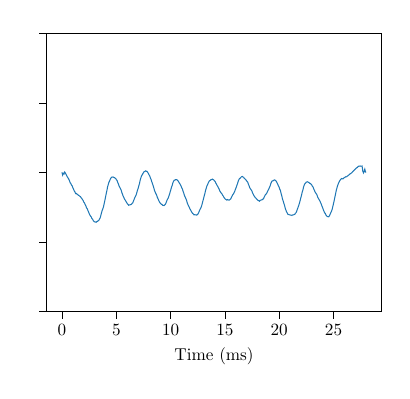
\begin{tikzpicture}[scale=0.62]

\definecolor{darkgray176}{RGB}{176,176,176}
\definecolor{steelblue31119180}{RGB}{31,119,180}

\begin{axis}[
yticklabel={\empty},
tick align=outside,
tick pos=left,
x grid style={darkgray176},
xlabel={Time (ms)},
xmin=-1.4, xmax=29.4,
xtick style={color=black},
y grid style={darkgray176},
% ylabel={Amplitude},
ymin=-0.1, ymax=0.1,
ytick style={color=black}
]
\addplot [semithick, steelblue31119180]
table {%
0 0
0.0626398210290828 -0.00193993691605009
0.125279642058166 -0.000697388132446564
0.187919463087248 -0.00111275092517369
0.250559284116331 0.00024235098553984
0.313199105145414 -0.000513447461112232
0.375838926174497 -0.00148002097020613
0.438478747203579 -0.00236590096614505
0.501118568232662 -0.00338719153914276
0.563758389261745 -0.0040478758738945
0.626398210290828 -0.00489145892378468
0.68903803131991 -0.00597273225852307
0.751677852348993 -0.0075518943669412
0.814317673378076 -0.00804388824375284
0.876957494407159 -0.00911086484564831
0.939597315436242 -0.00976522177482811
1.00223713646532 -0.0111615252149785
1.06487695749441 -0.0120892122812919
1.12751677852349 -0.0133643534484526
1.19015659955257 -0.0140450388668167
1.25279642058166 -0.0152411321678118
1.31543624161074 -0.0152015755478068
1.37807606263982 -0.0156972490801107
1.4407158836689 -0.0158916462787846
1.50335570469799 -0.0164657530043549
1.56599552572707 -0.0166319236784373
1.62863534675615 -0.0171322892138722
1.69127516778523 -0.0173743133176893
1.75391498881432 -0.0181628179505167
1.8165548098434 -0.0186722927520539
1.87919463087248 -0.0195240025227302
1.94183445190157 -0.0201793634176454
2.00447427293065 -0.0213767018969227
2.06711409395973 -0.0218668722441332
2.12975391498881 -0.0232046467170819
2.1923937360179 -0.0239699781816078
2.25503355704698 -0.0254819174265902
2.31767337807606 -0.0260842469514616
2.38031319910515 -0.02732341299021
2.44295302013423 -0.0283705943307821
2.50559284116331 -0.0296850969152363
2.56823266219239 -0.0306688831281542
2.63087248322148 -0.0315327634222355
2.69351230425056 -0.0320830301525409
2.75615212527964 -0.0332634595391534
2.81879194630872 -0.0337594674162617
2.88143176733781 -0.0346627948093134
2.94407158836689 -0.0353023716492341
3.00671140939597 -0.0356445175864352
3.06935123042506 -0.035673768940888
3.13199105145414 -0.0359154810516426
3.19463087248322 -0.035473047324375
3.2572706935123 -0.0353451175052648
3.31991051454139 -0.034851632399747
3.38255033557047 -0.0345895809540213
3.44519015659955 -0.0336693489436535
3.50782997762864 -0.0329108504115935
3.57046979865772 -0.0311585394228065
3.6331096196868 -0.0292167303671173
3.69574944071588 -0.0274955162390967
3.75838926174497 -0.0262148996452557
3.82102908277405 -0.0247058035468295
3.88366890380313 -0.0225165513962907
3.94630872483221 -0.0201710773344408
4.0089485458613 -0.0177496855815985
4.07158836689038 -0.015311727462799
4.13422818791946 -0.0130772745024238
4.19686800894855 -0.0104869296586754
4.25950782997763 -0.00871839223667079
4.32214765100671 -0.00709854418899389
4.38478747203579 -0.00616015045709858
4.44742729306488 -0.00491042862702536
4.51006711409396 -0.00406632385522927
4.57270693512304 -0.00346006396782878
4.63534675615213 -0.00342682171487968
4.69798657718121 -0.00326321851587135
4.76062639821029 -0.0036356184669089
4.82326621923937 -0.00375522114961539
4.88590604026846 -0.00417020489405466
4.94854586129754 -0.00445070286475172
5.01118568232662 -0.00530394186709551
5.0738255033557 -0.00580074416235989
5.13646532438479 -0.00734688157228216
5.19910514541387 -0.00843495169917009
5.26174496644295 -0.00992326142778933
5.32438478747204 -0.0108189789840839
5.38702460850112 -0.0118006604079832
5.4496644295302 -0.012858154283424
5.51230425055928 -0.0146084608847663
5.57494407158837 -0.0158316910629404
5.63758389261745 -0.017210534067462
5.70022371364653 -0.0182066267768809
5.76286353467562 -0.019341929859463
5.8255033557047 -0.0199633272827272
5.88814317673378 -0.0208683198805423
5.95078299776286 -0.0216582978656828
6.01342281879195 -0.022514550627878
6.07606263982103 -0.0229377234917159
6.13870246085011 -0.0236546001053296
6.2013422818792 -0.0234269479902199
6.26398210290828 -0.0233680328991789
6.32662192393736 -0.0231993186018811
6.38926174496644 -0.0230197730230405
6.45190156599553 -0.0223188432646078
6.51454138702461 -0.0219767539568195
6.57718120805369 -0.020686269068978
6.63982102908277 -0.0194335101959889
6.70246085011186 -0.0182000818543586
6.76510067114094 -0.0172540410328031
6.82774049217002 -0.016209368493983
6.89038031319911 -0.0145123920359668
6.95302013422819 -0.0128312964904928
7.01565995525727 -0.011369697843372
7.07829977628635 -0.00948762195497351
7.14093959731544 -0.00777829895358558
7.20357941834452 -0.00547778635167035
7.2662192393736 -0.00382289449815582
7.32885906040269 -0.00239693011538494
7.39149888143177 -0.001753756326417
7.45413870246085 -0.000781532301998778
7.51677852348993 6.73212836052733e-05
7.57941834451902 0.000587434764176407
7.6420581655481 0.000659656592163462
7.70469798657718 0.0011229761594894
7.76733780760626 0.000801310005704027
7.82997762863535 0.000698161930245841
7.89261744966443 -3.1259598447974e-05
7.95525727069351 -0.000749898274372888
8.0178970917226 -0.00186771298164889
8.08053691275168 -0.00256872730917179
8.14317673378076 -0.00407967935222507
8.20581655480984 -0.00523308175772228
8.26845637583893 -0.00684347297471242
8.33109619686801 -0.00807858403497094
8.39373601789709 -0.00967644710068735
8.45637583892617 -0.0112190790124388
8.51901565995526 -0.0130481103110133
8.58165548098434 -0.0142187896815922
8.64429530201342 -0.0153381289639229
8.70693512304251 -0.0162461492914281
8.76957494407159 -0.0178199395312359
8.83221476510067 -0.0188130948492545
8.89485458612975 -0.0201093304727302
8.95749440715884 -0.0210614237784339
9.02013422818792 -0.0218487176919143
9.082774049217 -0.0223928749461302
9.14541387024608 -0.0229616805836058
9.20805369127517 -0.0230043411204879
9.27069351230425 -0.0237804200475248
9.33333333333333 -0.0237110909074545
9.39597315436242 -0.0239102192248074
9.4586129753915 -0.0234278298964436
9.52125279642058 -0.0228990960941219
9.58389261744967 -0.0218231376360527
9.64653243847875 -0.0205061491703827
9.70917225950783 -0.0193424955160426
9.77181208053691 -0.018616105261065
9.834451901566 -0.0172838850146872
9.89709172259508 -0.0157916663439582
9.95973154362416 -0.0140185877930798
10.0223713646532 -0.0123708326644545
10.0850111856823 -0.0106744820552084
10.1476510067114 -0.00930849950285566
10.2102908277405 -0.00748266152812531
10.2729306487696 -0.00644440207655398
10.3355704697987 -0.00563968386776095
10.3982102908277 -0.00555548336881919
10.4608501118568 -0.00516599532991848
10.5234899328859 -0.0051542442767012
10.586129753915 -0.00529719335370816
10.6487695749441 -0.00593067748134568
10.7114093959732 -0.00634356388734691
10.7740492170022 -0.00736922608850986
10.8366890380313 -0.00803187458257147
10.8993288590604 -0.0089733005195056
10.9619686800895 -0.00978573921117807
11.0246085011186 -0.0111731671471924
11.0872483221477 -0.0119811839192806
11.1498881431767 -0.0137315380180742
11.2125279642058 -0.0149477422987455
11.2751677852349 -0.0166889945820174
11.337807606264 -0.0176660706157852
11.4004474272931 -0.0188565955391066
11.4630872483221 -0.0200510227040156
11.5257270693512 -0.0218445007633043
11.5883668903803 -0.0230041039145033
11.6510067114094 -0.0241762147278794
11.7136465324385 -0.0250530869718766
11.7762863534676 -0.0262797192714158
11.8389261744966 -0.027023786778918
11.9015659955257 -0.0280513898563265
11.9642058165548 -0.0288587481833544
12.0268456375839 -0.0295683772446925
12.089485458613 -0.0299139131960653
12.1521252796421 -0.0305846930675259
12.2147651006711 -0.0303976354407984
12.2774049217002 -0.0306569234711812
12.3400447427293 -0.0306414825179233
12.4026845637584 -0.0307158210608583
12.4653243847875 -0.0302266703306029
12.5279642058166 -0.0299377874815024
12.5906040268456 -0.0288169970173364
12.6532438478747 -0.0275692523850891
12.7158836689038 -0.0264562012115181
12.7785234899329 -0.0256634560857443
12.841163310962 -0.0244389498143788
12.9038031319911 -0.0226962687010133
12.9664429530201 -0.0207448930998377
13.0290827740492 -0.0189703644797106
13.0917225950783 -0.0169095892096626
13.1543624161074 -0.0151532614266112
13.2170022371365 -0.0129474857509536
13.2796420581655 -0.0113705251078378
13.3422818791946 -0.00967341267672561
13.4049217002237 -0.00875322164455116
13.4675615212528 -0.00757922379037478
13.5302013422819 -0.00659251304330842
13.592841163311 -0.00594735833122426
13.65548098434 -0.00570734011496873
13.7181208053691 -0.00515767018116961
13.7807606263982 -0.00519810113180804
13.8434004474273 -0.00482528749228324
13.9060402684564 -0.00515122189742807
13.9686800894855 -0.00544539820277851
14.0313199105145 -0.00606688503300984
14.0939597315436 -0.00646338295566556
14.1565995525727 -0.00763518456994687
14.2192393736018 -0.00843569395076109
14.2818791946309 -0.00947208871327391
14.34451901566 -0.0101807585123601
14.407158836689 -0.0111817509098441
14.4697986577181 -0.0120870489814638
14.5324384787472 -0.0134959457654681
14.5950782997763 -0.0141432432695323
14.6577181208054 -0.0148773754278085
14.7203579418345 -0.0154101146672596
14.7829977628635 -0.0163902547522979
14.8456375838926 -0.0170291740784809
14.9082774049217 -0.0179558711488975
14.9709172259508 -0.0186465589717131
15.0335570469799 -0.0192331361065575
15.0961968680089 -0.0195358479833043
15.158836689038 -0.0198954767078761
15.2214765100671 -0.0195587890710207
15.2841163310962 -0.0198893158277809
15.3467561521253 -0.0198336920307187
15.4093959731544 -0.019957424197721
15.4720357941834 -0.0194759885436737
15.5346756152125 -0.0190920362861564
15.5973154362416 -0.0180706887212176
15.6599552572707 -0.0169706257722722
15.7225950782998 -0.0159926750453427
15.7852348993289 -0.0154632865232509
15.8478747203579 -0.0145415439076672
15.910514541387 -0.0134155520069219
15.9731543624161 -0.0120827655164187
16.0357941834452 -0.0108127846263799
16.0984340044743 -0.00937753682018527
16.1610738255034 -0.0080538707716553
16.2237136465324 -0.00633208294892871
16.2863534675615 -0.00529039064234735
16.3489932885906 -0.00436794674086491
16.4116331096197 -0.00420468906253176
16.4742729306488 -0.0035372096170115
16.5369127516779 -0.00309298029982004
16.5995525727069 -0.00297285403256248
16.662192393736 -0.00334789148913134
16.7248322147651 -0.00356254867909339
16.7874720357942 -0.00435261607120101
16.8501118568233 -0.00472985238036853
16.9127516778523 -0.0053461461559238
16.9753914988814 -0.00567663938507138
17.0380313199105 -0.00658133582230782
17.1006711409396 -0.00707126775093927
17.1633109619687 -0.00855818980892233
17.2259507829978 -0.00963812948973387
17.2885906040268 -0.0111377743454087
17.3512304250559 -0.0117959981259184
17.413870246085 -0.0125579870737239
17.4765100671141 -0.0133017546953571
17.5391498881432 -0.0146937936094383
17.6017897091723 -0.0156262248329468
17.6644295302013 -0.0166750974553143
17.7270693512304 -0.0173641191420439
17.7897091722595 -0.0181859511532039
17.8523489932886 -0.0185211233469664
17.9149888143177 -0.0191185392139342
17.9776286353468 -0.0196192912482375
18.0402684563758 -0.0201465971517883
18.1029082774049 -0.0202752597405006
18.165548098434 -0.0207546639987486
18.2281879194631 -0.0202718090090976
18.2908277404922 -0.0199718117563917
18.3534675615213 -0.0198644418144386
18.4161073825503 -0.01982115804149
18.4787472035794 -0.0192898742779589
18.5413870246085 -0.0190784383515184
18.6040268456376 -0.0180081292961868
18.6666666666667 -0.0169898476451635
18.7293064876958 -0.0160652905727593
18.7919463087248 -0.0155984235977466
18.8545861297539 -0.0149188462719821
18.917225950783 -0.0138154529135099
18.9798657718121 -0.0127515262117822
19.0425055928412 -0.0119236599803971
19.1051454138702 -0.0107432210992947
19.1677852348993 -0.00963751154157939
19.2304250559284 -0.00792205298706989
19.2930648769575 -0.00688576142009873
19.3557046979866 -0.00610579497137126
19.4183445190157 -0.0061797442214701
19.4809843400447 -0.00575651343436849
19.5436241610738 -0.00549986924751093
19.6062639821029 -0.00550226312155691
19.668903803132 -0.00602696132189875
19.7315436241611 -0.00635458142090364
19.7941834451902 -0.00754223414540491
19.8568232662192 -0.0084792148796904
19.9194630872483 -0.00964791891508854
19.9821029082774 -0.0105099868554397
20.0447427293065 -0.0120551966680776
20.1073825503356 -0.0130137496271589
20.1700223713647 -0.0152044488717146
20.2326621923937 -0.0168635845809375
20.2953020134228 -0.019133672555721
20.3579418344519 -0.0205623124469847
20.420581655481 -0.0221308947309552
20.4832214765101 -0.0235966664532687
20.5458612975392 -0.0256366451089614
20.6085011185682 -0.0270639085054598
20.6711409395973 -0.0283343148286511
20.7337807606264 -0.0291837782492774
20.7964205816555 -0.0301544365391835
20.8590604026846 -0.0303579606990886
20.9217002237136 -0.0305262249863188
20.9843400447427 -0.0306423743249186
21.0469798657718 -0.0307146397438025
21.1096196868009 -0.0307650097689573
21.17225950783 -0.0310371947543533
21.2348993288591 -0.0305777494889378
21.2975391498881 -0.0306150344319192
21.3601789709172 -0.0303580903591926
21.4228187919463 -0.0302442793903135
21.4854586129754 -0.0294810385637035
21.5480984340045 -0.0290137161719519
21.6107382550336 -0.0278098889870332
21.6733780760626 -0.0264089604177131
21.7360178970917 -0.0250087135765176
21.7986577181208 -0.0237058942524979
21.8612975391499 -0.0220596348279275
21.923937360179 -0.02028223028369
21.9865771812081 -0.0182890103592369
22.0492170022371 -0.0164573208847702
22.1118568232662 -0.0143455547724394
22.1744966442953 -0.0127747641413804
22.2371364653244 -0.010639312633332
22.2997762863535 -0.00914210952418363
22.3624161073826 -0.00808671373723937
22.4250559284116 -0.00765494831006399
22.4876957494407 -0.00705658045016079
22.5503355704698 -0.00685571037832923
22.6129753914989 -0.00677605473355159
22.675615212528 -0.00717133541760229
22.738255033557 -0.00729907692828834
22.8008948545861 -0.00784356573334076
22.8635346756152 -0.00799461079748885
22.9261744966443 -0.00850925071402484
22.9888143176734 -0.00898205096389623
23.0514541387025 -0.00996084994442711
23.1140939597315 -0.0106121865944974
23.1767337807606 -0.0119826560777506
23.2393736017897 -0.0128798367418099
23.3020134228188 -0.01422062497461
23.3646532438479 -0.0148710731429442
23.427293064877 -0.0156335985325527
23.489932885906 -0.0165303014281312
23.5525727069351 -0.018088021696914
23.6152125279642 -0.0188820565231894
23.6778523489933 -0.0197612943265262
23.7404921700224 -0.0205219524143726
23.8031319910515 -0.0217698877864836
23.8657718120805 -0.0227528209079232
23.9284116331096 -0.024208398373335
23.9910514541387 -0.0253864640632532
24.0536912751678 -0.0268292097662319
24.1163310961969 -0.0279409261732893
24.1789709172259 -0.0291731259191796
24.241610738255 -0.0295585168888105
24.3042505592841 -0.0308126008525591
24.3668903803132 -0.031327838678188
24.4295302013423 -0.0318774218177235
24.4921700223714 -0.0318811046422128
24.5548098434004 -0.0319863388802381
24.6174496644295 -0.0312568510463774
24.6800894854586 -0.0302467762098816
24.7427293064877 -0.0290509528111691
24.8053691275168 -0.0280506531364166
24.8680089485459 -0.0266603137047699
24.9306487695749 -0.0246157685932297
24.993288590604 -0.0225176575324879
25.0559284116331 -0.0203431202786281
25.1185682326622 -0.0178945301813167
25.1812080536913 -0.0156796480335245
25.2438478747204 -0.0131607170047976
25.3064876957494 -0.0113573145908897
25.3691275167785 -0.00954080660571188
25.4317673378076 -0.0083261649030567
25.4944071588367 -0.00708915283215926
25.5570469798658 -0.00624982667649352
25.6196868008949 -0.00537700829839946
25.6823266219239 -0.00494568711209217
25.744966442953 -0.00445876410543519
25.8076062639821 -0.00463843895684953
25.8702460850112 -0.00463734595917615
25.9328859060403 -0.00417199610863756
25.9955257270694 -0.00376390583263148
26.0581655480984 -0.00351306192276862
26.1208053691275 -0.00316015437195365
26.1834451901566 -0.00319486327669365
26.2460850111857 -0.0028069100573959
26.3087248322148 -0.00251574174269734
26.3713646532438 -0.00206075192447877
26.4340044742729 -0.00175063678332223
26.496644295302 -0.00115453855653337
26.5592841163311 -0.000961863192035849
26.6219239373602 -0.000519481618832422
26.6845637583893 -0.000253477640099975
26.7472035794183 0.000386290302212607
26.8098434004474 0.000813860121189346
26.8724832214765 0.00136720877915821
26.9351230425056 0.00177161288041396
26.9977628635347 0.0023945276094163
27.0604026845638 0.0027713477986571
27.1230425055928 0.00326533768101027
27.1856823266219 0.00345150310071123
27.248322147651 0.00407087321599458
27.3109619686801 0.00446927401193436
27.3736017897092 0.00457032027360577
27.4362416107383 0.00441366212830047
27.4988814317673 0.00459057578954521
27.5615212527964 0.00445979537329818
27.6241610738255 0.00456084163496958
27.6868008948546 0.00105147996304819
27.7494407158837 -0.000385981415642188
27.8120805369128 0.00072438754891389
27.8747203579418 0.00228477716945962
27.9373601789709 0.00025185048830189
28 0
};
\end{axis}

\end{tikzpicture}

	\end{subfigure}\hfill
	\begin{subfigure}{0.3\textwidth}
		\centering
		% This file was created with tikzplotlib v0.10.1.
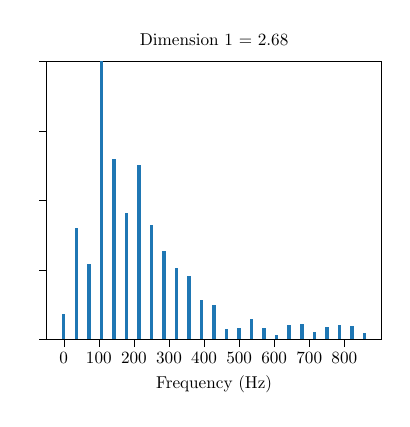
\begin{tikzpicture}[scale=0.62]

\definecolor{darkgray176}{RGB}{176,176,176}
\definecolor{steelblue31119180}{RGB}{31,119,180}

\begin{axis}[
yticklabel={\empty},
tick align=outside,
tick pos=left,
x grid style={darkgray176},
xlabel={Frequency (Hz)},
xmin=-48.3571428571429, xmax=905.5,
xtick style={color=black},
xtick={0, 100, 200, 300, 400, 500, 600, 700, 800}, % Set explicit tick positions
y grid style={darkgray176},
%ylabel={Magnitude},
ymin=0, ymax=4,
title={Dimension 1 = 2.68},
ytick style={color=black}
]
\draw[draw=none,fill=steelblue31119180] (axis cs:-5,0) rectangle (axis cs:5,0.363293109461665);
\draw[draw=none,fill=steelblue31119180] (axis cs:30.7142857142857,0) rectangle (axis cs:40.7142857142857,1.59671692845371);
\draw[draw=none,fill=steelblue31119180] (axis cs:66.4285714285714,0) rectangle (axis cs:76.4285714285714,1.08375129075336);
\draw[draw=none,fill=steelblue31119180] (axis cs:102.142857142857,0) rectangle (axis cs:112.142857142857,5.72028640718505);
\draw[draw=none,fill=steelblue31119180] (axis cs:137.857142857143,0) rectangle (axis cs:147.857142857143,2.60109171070077);
\draw[draw=none,fill=steelblue31119180] (axis cs:173.571428571429,0) rectangle (axis cs:183.571428571429,1.82230187959835);
\draw[draw=none,fill=steelblue31119180] (axis cs:209.285714285714,0) rectangle (axis cs:219.285714285714,2.50466396839656);
\draw[draw=none,fill=steelblue31119180] (axis cs:245,0) rectangle (axis cs:255,1.64154431128106);
\draw[draw=none,fill=steelblue31119180] (axis cs:280.714285714286,0) rectangle (axis cs:290.714285714286,1.2779936763853);
\draw[draw=none,fill=steelblue31119180] (axis cs:316.428571428571,0) rectangle (axis cs:326.428571428571,1.02566988726104);
\draw[draw=none,fill=steelblue31119180] (axis cs:352.142857142857,0) rectangle (axis cs:362.142857142857,0.906444113984638);
\draw[draw=none,fill=steelblue31119180] (axis cs:387.857142857143,0) rectangle (axis cs:397.857142857143,0.567573738688084);
\draw[draw=none,fill=steelblue31119180] (axis cs:423.571428571429,0) rectangle (axis cs:433.571428571429,0.497884322563813);
\draw[draw=none,fill=steelblue31119180] (axis cs:459.285714285714,0) rectangle (axis cs:469.285714285714,0.143370970638671);
\draw[draw=none,fill=steelblue31119180] (axis cs:495,0) rectangle (axis cs:505,0.158030205491621);
\draw[draw=none,fill=steelblue31119180] (axis cs:530.714285714286,0) rectangle (axis cs:540.714285714286,0.287791882784369);
\draw[draw=none,fill=steelblue31119180] (axis cs:566.428571428571,0) rectangle (axis cs:576.428571428571,0.164560600100172);
\draw[draw=none,fill=steelblue31119180] (axis cs:602.142857142857,0) rectangle (axis cs:612.142857142857,0.0653538748355305);
\draw[draw=none,fill=steelblue31119180] (axis cs:637.857142857143,0) rectangle (axis cs:647.857142857143,0.209706204538538);
\draw[draw=none,fill=steelblue31119180] (axis cs:673.571428571429,0) rectangle (axis cs:683.571428571429,0.216581742305538);
\draw[draw=none,fill=steelblue31119180] (axis cs:709.285714285714,0) rectangle (axis cs:719.285714285714,0.104565114650486);
\draw[draw=none,fill=steelblue31119180] (axis cs:745,0) rectangle (axis cs:755,0.18370350932939);
\draw[draw=none,fill=steelblue31119180] (axis cs:780.714285714286,0) rectangle (axis cs:790.714285714286,0.206670350113575);
\draw[draw=none,fill=steelblue31119180] (axis cs:816.428571428571,0) rectangle (axis cs:826.428571428571,0.196489132073225);
\draw[draw=none,fill=steelblue31119180] (axis cs:852.142857142857,0) rectangle (axis cs:862.142857142857,0.0885177801919891);
\end{axis}

\end{tikzpicture}

	\end{subfigure}
	
	\vspace{0.5cm} % Adjust vertical spacing between rows
	
	\begin{subfigure}{0.36\textwidth}
		\centering
		% This file was created with tikzplotlib v0.10.1.
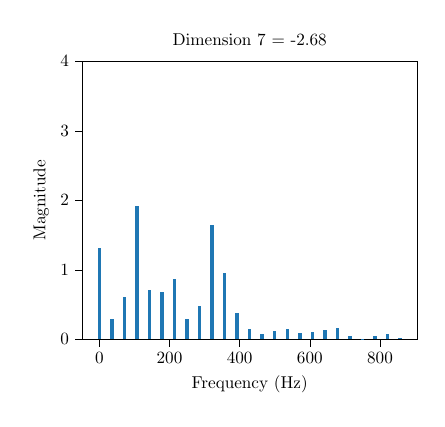
\begin{tikzpicture}[scale=0.62]

\definecolor{darkgray176}{RGB}{176,176,176}
\definecolor{steelblue31119180}{RGB}{31,119,180}

\begin{axis}[
tick align=outside,
tick pos=left,
x grid style={darkgray176},
xlabel={Frequency (Hz)},
xmin=-48.3571428571429, xmax=905.5,
xtick style={color=black},
y grid style={darkgray176},
ylabel={Magnitude},
ymin=0, ymax=4,
title={Dimension 7 = -2.68},
ytick style={color=black}
]
\draw[draw=none,fill=steelblue31119180] (axis cs:-5,0) rectangle (axis cs:5,1.31270937714726);
\draw[draw=none,fill=steelblue31119180] (axis cs:30.7142857142857,0) rectangle (axis cs:40.7142857142857,0.288125975872221);
\draw[draw=none,fill=steelblue31119180] (axis cs:66.4285714285714,0) rectangle (axis cs:76.4285714285714,0.616790952368152);
\draw[draw=none,fill=steelblue31119180] (axis cs:102.142857142857,0) rectangle (axis cs:112.142857142857,1.92312523138079);
\draw[draw=none,fill=steelblue31119180] (axis cs:137.857142857143,0) rectangle (axis cs:147.857142857143,0.707237007629874);
\draw[draw=none,fill=steelblue31119180] (axis cs:173.571428571429,0) rectangle (axis cs:183.571428571429,0.677698119881814);
\draw[draw=none,fill=steelblue31119180] (axis cs:209.285714285714,0) rectangle (axis cs:219.285714285714,0.862386040544995);
\draw[draw=none,fill=steelblue31119180] (axis cs:245,0) rectangle (axis cs:255,0.298711415685218);
\draw[draw=none,fill=steelblue31119180] (axis cs:280.714285714286,0) rectangle (axis cs:290.714285714286,0.483968708976862);
\draw[draw=none,fill=steelblue31119180] (axis cs:316.428571428571,0) rectangle (axis cs:326.428571428571,1.65269155101225);
\draw[draw=none,fill=steelblue31119180] (axis cs:352.142857142857,0) rectangle (axis cs:362.142857142857,0.951122100407993);
\draw[draw=none,fill=steelblue31119180] (axis cs:387.857142857143,0) rectangle (axis cs:397.857142857143,0.377021033569998);
\draw[draw=none,fill=steelblue31119180] (axis cs:423.571428571429,0) rectangle (axis cs:433.571428571429,0.156449857538637);
\draw[draw=none,fill=steelblue31119180] (axis cs:459.285714285714,0) rectangle (axis cs:469.285714285714,0.0846393619854383);
\draw[draw=none,fill=steelblue31119180] (axis cs:495,0) rectangle (axis cs:505,0.118818944486802);
\draw[draw=none,fill=steelblue31119180] (axis cs:530.714285714286,0) rectangle (axis cs:540.714285714286,0.143214948815801);
\draw[draw=none,fill=steelblue31119180] (axis cs:566.428571428571,0) rectangle (axis cs:576.428571428571,0.0949080699867579);
\draw[draw=none,fill=steelblue31119180] (axis cs:602.142857142857,0) rectangle (axis cs:612.142857142857,0.10757439472035);
\draw[draw=none,fill=steelblue31119180] (axis cs:637.857142857143,0) rectangle (axis cs:647.857142857143,0.131395993038413);
\draw[draw=none,fill=steelblue31119180] (axis cs:673.571428571429,0) rectangle (axis cs:683.571428571429,0.160127533802761);
\draw[draw=none,fill=steelblue31119180] (axis cs:709.285714285714,0) rectangle (axis cs:719.285714285714,0.0535699464522896);
\draw[draw=none,fill=steelblue31119180] (axis cs:745,0) rectangle (axis cs:755,0.00967304476823895);
\draw[draw=none,fill=steelblue31119180] (axis cs:780.714285714286,0) rectangle (axis cs:790.714285714286,0.0422317493349039);
\draw[draw=none,fill=steelblue31119180] (axis cs:816.428571428571,0) rectangle (axis cs:826.428571428571,0.0743497564419976);
\draw[draw=none,fill=steelblue31119180] (axis cs:852.142857142857,0) rectangle (axis cs:862.142857142857,0.0273048386393424);
\end{axis}

\end{tikzpicture}

	\end{subfigure}\hfill
	\begin{subfigure}{0.3\textwidth}
		\centering
		% This file was created with tikzplotlib v0.10.1.
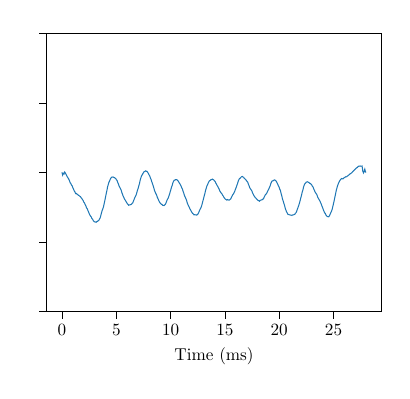
\begin{tikzpicture}[scale=0.62]

\definecolor{darkgray176}{RGB}{176,176,176}
\definecolor{steelblue31119180}{RGB}{31,119,180}

\begin{axis}[
yticklabel={\empty},
tick align=outside,
tick pos=left,
x grid style={darkgray176},
xlabel={Time (ms)},
xmin=-1.4, xmax=29.4,
xtick style={color=black},
y grid style={darkgray176},
% ylabel={Amplitude},
ymin=-0.1, ymax=0.1,
ytick style={color=black}
]
\addplot [semithick, steelblue31119180]
table {%
0 0
0.0626398210290828 -0.00193993691605009
0.125279642058166 -0.000697388132446564
0.187919463087248 -0.00111275092517369
0.250559284116331 0.00024235098553984
0.313199105145414 -0.000513447461112232
0.375838926174497 -0.00148002097020613
0.438478747203579 -0.00236590096614505
0.501118568232662 -0.00338719153914276
0.563758389261745 -0.0040478758738945
0.626398210290828 -0.00489145892378468
0.68903803131991 -0.00597273225852307
0.751677852348993 -0.0075518943669412
0.814317673378076 -0.00804388824375284
0.876957494407159 -0.00911086484564831
0.939597315436242 -0.00976522177482811
1.00223713646532 -0.0111615252149785
1.06487695749441 -0.0120892122812919
1.12751677852349 -0.0133643534484526
1.19015659955257 -0.0140450388668167
1.25279642058166 -0.0152411321678118
1.31543624161074 -0.0152015755478068
1.37807606263982 -0.0156972490801107
1.4407158836689 -0.0158916462787846
1.50335570469799 -0.0164657530043549
1.56599552572707 -0.0166319236784373
1.62863534675615 -0.0171322892138722
1.69127516778523 -0.0173743133176893
1.75391498881432 -0.0181628179505167
1.8165548098434 -0.0186722927520539
1.87919463087248 -0.0195240025227302
1.94183445190157 -0.0201793634176454
2.00447427293065 -0.0213767018969227
2.06711409395973 -0.0218668722441332
2.12975391498881 -0.0232046467170819
2.1923937360179 -0.0239699781816078
2.25503355704698 -0.0254819174265902
2.31767337807606 -0.0260842469514616
2.38031319910515 -0.02732341299021
2.44295302013423 -0.0283705943307821
2.50559284116331 -0.0296850969152363
2.56823266219239 -0.0306688831281542
2.63087248322148 -0.0315327634222355
2.69351230425056 -0.0320830301525409
2.75615212527964 -0.0332634595391534
2.81879194630872 -0.0337594674162617
2.88143176733781 -0.0346627948093134
2.94407158836689 -0.0353023716492341
3.00671140939597 -0.0356445175864352
3.06935123042506 -0.035673768940888
3.13199105145414 -0.0359154810516426
3.19463087248322 -0.035473047324375
3.2572706935123 -0.0353451175052648
3.31991051454139 -0.034851632399747
3.38255033557047 -0.0345895809540213
3.44519015659955 -0.0336693489436535
3.50782997762864 -0.0329108504115935
3.57046979865772 -0.0311585394228065
3.6331096196868 -0.0292167303671173
3.69574944071588 -0.0274955162390967
3.75838926174497 -0.0262148996452557
3.82102908277405 -0.0247058035468295
3.88366890380313 -0.0225165513962907
3.94630872483221 -0.0201710773344408
4.0089485458613 -0.0177496855815985
4.07158836689038 -0.015311727462799
4.13422818791946 -0.0130772745024238
4.19686800894855 -0.0104869296586754
4.25950782997763 -0.00871839223667079
4.32214765100671 -0.00709854418899389
4.38478747203579 -0.00616015045709858
4.44742729306488 -0.00491042862702536
4.51006711409396 -0.00406632385522927
4.57270693512304 -0.00346006396782878
4.63534675615213 -0.00342682171487968
4.69798657718121 -0.00326321851587135
4.76062639821029 -0.0036356184669089
4.82326621923937 -0.00375522114961539
4.88590604026846 -0.00417020489405466
4.94854586129754 -0.00445070286475172
5.01118568232662 -0.00530394186709551
5.0738255033557 -0.00580074416235989
5.13646532438479 -0.00734688157228216
5.19910514541387 -0.00843495169917009
5.26174496644295 -0.00992326142778933
5.32438478747204 -0.0108189789840839
5.38702460850112 -0.0118006604079832
5.4496644295302 -0.012858154283424
5.51230425055928 -0.0146084608847663
5.57494407158837 -0.0158316910629404
5.63758389261745 -0.017210534067462
5.70022371364653 -0.0182066267768809
5.76286353467562 -0.019341929859463
5.8255033557047 -0.0199633272827272
5.88814317673378 -0.0208683198805423
5.95078299776286 -0.0216582978656828
6.01342281879195 -0.022514550627878
6.07606263982103 -0.0229377234917159
6.13870246085011 -0.0236546001053296
6.2013422818792 -0.0234269479902199
6.26398210290828 -0.0233680328991789
6.32662192393736 -0.0231993186018811
6.38926174496644 -0.0230197730230405
6.45190156599553 -0.0223188432646078
6.51454138702461 -0.0219767539568195
6.57718120805369 -0.020686269068978
6.63982102908277 -0.0194335101959889
6.70246085011186 -0.0182000818543586
6.76510067114094 -0.0172540410328031
6.82774049217002 -0.016209368493983
6.89038031319911 -0.0145123920359668
6.95302013422819 -0.0128312964904928
7.01565995525727 -0.011369697843372
7.07829977628635 -0.00948762195497351
7.14093959731544 -0.00777829895358558
7.20357941834452 -0.00547778635167035
7.2662192393736 -0.00382289449815582
7.32885906040269 -0.00239693011538494
7.39149888143177 -0.001753756326417
7.45413870246085 -0.000781532301998778
7.51677852348993 6.73212836052733e-05
7.57941834451902 0.000587434764176407
7.6420581655481 0.000659656592163462
7.70469798657718 0.0011229761594894
7.76733780760626 0.000801310005704027
7.82997762863535 0.000698161930245841
7.89261744966443 -3.1259598447974e-05
7.95525727069351 -0.000749898274372888
8.0178970917226 -0.00186771298164889
8.08053691275168 -0.00256872730917179
8.14317673378076 -0.00407967935222507
8.20581655480984 -0.00523308175772228
8.26845637583893 -0.00684347297471242
8.33109619686801 -0.00807858403497094
8.39373601789709 -0.00967644710068735
8.45637583892617 -0.0112190790124388
8.51901565995526 -0.0130481103110133
8.58165548098434 -0.0142187896815922
8.64429530201342 -0.0153381289639229
8.70693512304251 -0.0162461492914281
8.76957494407159 -0.0178199395312359
8.83221476510067 -0.0188130948492545
8.89485458612975 -0.0201093304727302
8.95749440715884 -0.0210614237784339
9.02013422818792 -0.0218487176919143
9.082774049217 -0.0223928749461302
9.14541387024608 -0.0229616805836058
9.20805369127517 -0.0230043411204879
9.27069351230425 -0.0237804200475248
9.33333333333333 -0.0237110909074545
9.39597315436242 -0.0239102192248074
9.4586129753915 -0.0234278298964436
9.52125279642058 -0.0228990960941219
9.58389261744967 -0.0218231376360527
9.64653243847875 -0.0205061491703827
9.70917225950783 -0.0193424955160426
9.77181208053691 -0.018616105261065
9.834451901566 -0.0172838850146872
9.89709172259508 -0.0157916663439582
9.95973154362416 -0.0140185877930798
10.0223713646532 -0.0123708326644545
10.0850111856823 -0.0106744820552084
10.1476510067114 -0.00930849950285566
10.2102908277405 -0.00748266152812531
10.2729306487696 -0.00644440207655398
10.3355704697987 -0.00563968386776095
10.3982102908277 -0.00555548336881919
10.4608501118568 -0.00516599532991848
10.5234899328859 -0.0051542442767012
10.586129753915 -0.00529719335370816
10.6487695749441 -0.00593067748134568
10.7114093959732 -0.00634356388734691
10.7740492170022 -0.00736922608850986
10.8366890380313 -0.00803187458257147
10.8993288590604 -0.0089733005195056
10.9619686800895 -0.00978573921117807
11.0246085011186 -0.0111731671471924
11.0872483221477 -0.0119811839192806
11.1498881431767 -0.0137315380180742
11.2125279642058 -0.0149477422987455
11.2751677852349 -0.0166889945820174
11.337807606264 -0.0176660706157852
11.4004474272931 -0.0188565955391066
11.4630872483221 -0.0200510227040156
11.5257270693512 -0.0218445007633043
11.5883668903803 -0.0230041039145033
11.6510067114094 -0.0241762147278794
11.7136465324385 -0.0250530869718766
11.7762863534676 -0.0262797192714158
11.8389261744966 -0.027023786778918
11.9015659955257 -0.0280513898563265
11.9642058165548 -0.0288587481833544
12.0268456375839 -0.0295683772446925
12.089485458613 -0.0299139131960653
12.1521252796421 -0.0305846930675259
12.2147651006711 -0.0303976354407984
12.2774049217002 -0.0306569234711812
12.3400447427293 -0.0306414825179233
12.4026845637584 -0.0307158210608583
12.4653243847875 -0.0302266703306029
12.5279642058166 -0.0299377874815024
12.5906040268456 -0.0288169970173364
12.6532438478747 -0.0275692523850891
12.7158836689038 -0.0264562012115181
12.7785234899329 -0.0256634560857443
12.841163310962 -0.0244389498143788
12.9038031319911 -0.0226962687010133
12.9664429530201 -0.0207448930998377
13.0290827740492 -0.0189703644797106
13.0917225950783 -0.0169095892096626
13.1543624161074 -0.0151532614266112
13.2170022371365 -0.0129474857509536
13.2796420581655 -0.0113705251078378
13.3422818791946 -0.00967341267672561
13.4049217002237 -0.00875322164455116
13.4675615212528 -0.00757922379037478
13.5302013422819 -0.00659251304330842
13.592841163311 -0.00594735833122426
13.65548098434 -0.00570734011496873
13.7181208053691 -0.00515767018116961
13.7807606263982 -0.00519810113180804
13.8434004474273 -0.00482528749228324
13.9060402684564 -0.00515122189742807
13.9686800894855 -0.00544539820277851
14.0313199105145 -0.00606688503300984
14.0939597315436 -0.00646338295566556
14.1565995525727 -0.00763518456994687
14.2192393736018 -0.00843569395076109
14.2818791946309 -0.00947208871327391
14.34451901566 -0.0101807585123601
14.407158836689 -0.0111817509098441
14.4697986577181 -0.0120870489814638
14.5324384787472 -0.0134959457654681
14.5950782997763 -0.0141432432695323
14.6577181208054 -0.0148773754278085
14.7203579418345 -0.0154101146672596
14.7829977628635 -0.0163902547522979
14.8456375838926 -0.0170291740784809
14.9082774049217 -0.0179558711488975
14.9709172259508 -0.0186465589717131
15.0335570469799 -0.0192331361065575
15.0961968680089 -0.0195358479833043
15.158836689038 -0.0198954767078761
15.2214765100671 -0.0195587890710207
15.2841163310962 -0.0198893158277809
15.3467561521253 -0.0198336920307187
15.4093959731544 -0.019957424197721
15.4720357941834 -0.0194759885436737
15.5346756152125 -0.0190920362861564
15.5973154362416 -0.0180706887212176
15.6599552572707 -0.0169706257722722
15.7225950782998 -0.0159926750453427
15.7852348993289 -0.0154632865232509
15.8478747203579 -0.0145415439076672
15.910514541387 -0.0134155520069219
15.9731543624161 -0.0120827655164187
16.0357941834452 -0.0108127846263799
16.0984340044743 -0.00937753682018527
16.1610738255034 -0.0080538707716553
16.2237136465324 -0.00633208294892871
16.2863534675615 -0.00529039064234735
16.3489932885906 -0.00436794674086491
16.4116331096197 -0.00420468906253176
16.4742729306488 -0.0035372096170115
16.5369127516779 -0.00309298029982004
16.5995525727069 -0.00297285403256248
16.662192393736 -0.00334789148913134
16.7248322147651 -0.00356254867909339
16.7874720357942 -0.00435261607120101
16.8501118568233 -0.00472985238036853
16.9127516778523 -0.0053461461559238
16.9753914988814 -0.00567663938507138
17.0380313199105 -0.00658133582230782
17.1006711409396 -0.00707126775093927
17.1633109619687 -0.00855818980892233
17.2259507829978 -0.00963812948973387
17.2885906040268 -0.0111377743454087
17.3512304250559 -0.0117959981259184
17.413870246085 -0.0125579870737239
17.4765100671141 -0.0133017546953571
17.5391498881432 -0.0146937936094383
17.6017897091723 -0.0156262248329468
17.6644295302013 -0.0166750974553143
17.7270693512304 -0.0173641191420439
17.7897091722595 -0.0181859511532039
17.8523489932886 -0.0185211233469664
17.9149888143177 -0.0191185392139342
17.9776286353468 -0.0196192912482375
18.0402684563758 -0.0201465971517883
18.1029082774049 -0.0202752597405006
18.165548098434 -0.0207546639987486
18.2281879194631 -0.0202718090090976
18.2908277404922 -0.0199718117563917
18.3534675615213 -0.0198644418144386
18.4161073825503 -0.01982115804149
18.4787472035794 -0.0192898742779589
18.5413870246085 -0.0190784383515184
18.6040268456376 -0.0180081292961868
18.6666666666667 -0.0169898476451635
18.7293064876958 -0.0160652905727593
18.7919463087248 -0.0155984235977466
18.8545861297539 -0.0149188462719821
18.917225950783 -0.0138154529135099
18.9798657718121 -0.0127515262117822
19.0425055928412 -0.0119236599803971
19.1051454138702 -0.0107432210992947
19.1677852348993 -0.00963751154157939
19.2304250559284 -0.00792205298706989
19.2930648769575 -0.00688576142009873
19.3557046979866 -0.00610579497137126
19.4183445190157 -0.0061797442214701
19.4809843400447 -0.00575651343436849
19.5436241610738 -0.00549986924751093
19.6062639821029 -0.00550226312155691
19.668903803132 -0.00602696132189875
19.7315436241611 -0.00635458142090364
19.7941834451902 -0.00754223414540491
19.8568232662192 -0.0084792148796904
19.9194630872483 -0.00964791891508854
19.9821029082774 -0.0105099868554397
20.0447427293065 -0.0120551966680776
20.1073825503356 -0.0130137496271589
20.1700223713647 -0.0152044488717146
20.2326621923937 -0.0168635845809375
20.2953020134228 -0.019133672555721
20.3579418344519 -0.0205623124469847
20.420581655481 -0.0221308947309552
20.4832214765101 -0.0235966664532687
20.5458612975392 -0.0256366451089614
20.6085011185682 -0.0270639085054598
20.6711409395973 -0.0283343148286511
20.7337807606264 -0.0291837782492774
20.7964205816555 -0.0301544365391835
20.8590604026846 -0.0303579606990886
20.9217002237136 -0.0305262249863188
20.9843400447427 -0.0306423743249186
21.0469798657718 -0.0307146397438025
21.1096196868009 -0.0307650097689573
21.17225950783 -0.0310371947543533
21.2348993288591 -0.0305777494889378
21.2975391498881 -0.0306150344319192
21.3601789709172 -0.0303580903591926
21.4228187919463 -0.0302442793903135
21.4854586129754 -0.0294810385637035
21.5480984340045 -0.0290137161719519
21.6107382550336 -0.0278098889870332
21.6733780760626 -0.0264089604177131
21.7360178970917 -0.0250087135765176
21.7986577181208 -0.0237058942524979
21.8612975391499 -0.0220596348279275
21.923937360179 -0.02028223028369
21.9865771812081 -0.0182890103592369
22.0492170022371 -0.0164573208847702
22.1118568232662 -0.0143455547724394
22.1744966442953 -0.0127747641413804
22.2371364653244 -0.010639312633332
22.2997762863535 -0.00914210952418363
22.3624161073826 -0.00808671373723937
22.4250559284116 -0.00765494831006399
22.4876957494407 -0.00705658045016079
22.5503355704698 -0.00685571037832923
22.6129753914989 -0.00677605473355159
22.675615212528 -0.00717133541760229
22.738255033557 -0.00729907692828834
22.8008948545861 -0.00784356573334076
22.8635346756152 -0.00799461079748885
22.9261744966443 -0.00850925071402484
22.9888143176734 -0.00898205096389623
23.0514541387025 -0.00996084994442711
23.1140939597315 -0.0106121865944974
23.1767337807606 -0.0119826560777506
23.2393736017897 -0.0128798367418099
23.3020134228188 -0.01422062497461
23.3646532438479 -0.0148710731429442
23.427293064877 -0.0156335985325527
23.489932885906 -0.0165303014281312
23.5525727069351 -0.018088021696914
23.6152125279642 -0.0188820565231894
23.6778523489933 -0.0197612943265262
23.7404921700224 -0.0205219524143726
23.8031319910515 -0.0217698877864836
23.8657718120805 -0.0227528209079232
23.9284116331096 -0.024208398373335
23.9910514541387 -0.0253864640632532
24.0536912751678 -0.0268292097662319
24.1163310961969 -0.0279409261732893
24.1789709172259 -0.0291731259191796
24.241610738255 -0.0295585168888105
24.3042505592841 -0.0308126008525591
24.3668903803132 -0.031327838678188
24.4295302013423 -0.0318774218177235
24.4921700223714 -0.0318811046422128
24.5548098434004 -0.0319863388802381
24.6174496644295 -0.0312568510463774
24.6800894854586 -0.0302467762098816
24.7427293064877 -0.0290509528111691
24.8053691275168 -0.0280506531364166
24.8680089485459 -0.0266603137047699
24.9306487695749 -0.0246157685932297
24.993288590604 -0.0225176575324879
25.0559284116331 -0.0203431202786281
25.1185682326622 -0.0178945301813167
25.1812080536913 -0.0156796480335245
25.2438478747204 -0.0131607170047976
25.3064876957494 -0.0113573145908897
25.3691275167785 -0.00954080660571188
25.4317673378076 -0.0083261649030567
25.4944071588367 -0.00708915283215926
25.5570469798658 -0.00624982667649352
25.6196868008949 -0.00537700829839946
25.6823266219239 -0.00494568711209217
25.744966442953 -0.00445876410543519
25.8076062639821 -0.00463843895684953
25.8702460850112 -0.00463734595917615
25.9328859060403 -0.00417199610863756
25.9955257270694 -0.00376390583263148
26.0581655480984 -0.00351306192276862
26.1208053691275 -0.00316015437195365
26.1834451901566 -0.00319486327669365
26.2460850111857 -0.0028069100573959
26.3087248322148 -0.00251574174269734
26.3713646532438 -0.00206075192447877
26.4340044742729 -0.00175063678332223
26.496644295302 -0.00115453855653337
26.5592841163311 -0.000961863192035849
26.6219239373602 -0.000519481618832422
26.6845637583893 -0.000253477640099975
26.7472035794183 0.000386290302212607
26.8098434004474 0.000813860121189346
26.8724832214765 0.00136720877915821
26.9351230425056 0.00177161288041396
26.9977628635347 0.0023945276094163
27.0604026845638 0.0027713477986571
27.1230425055928 0.00326533768101027
27.1856823266219 0.00345150310071123
27.248322147651 0.00407087321599458
27.3109619686801 0.00446927401193436
27.3736017897092 0.00457032027360577
27.4362416107383 0.00441366212830047
27.4988814317673 0.00459057578954521
27.5615212527964 0.00445979537329818
27.6241610738255 0.00456084163496958
27.6868008948546 0.00105147996304819
27.7494407158837 -0.000385981415642188
27.8120805369128 0.00072438754891389
27.8747203579418 0.00228477716945962
27.9373601789709 0.00025185048830189
28 0
};
\end{axis}

\end{tikzpicture}

	\end{subfigure}\hfill
	\begin{subfigure}{0.3\textwidth}
		\centering
		% This file was created with tikzplotlib v0.10.1.
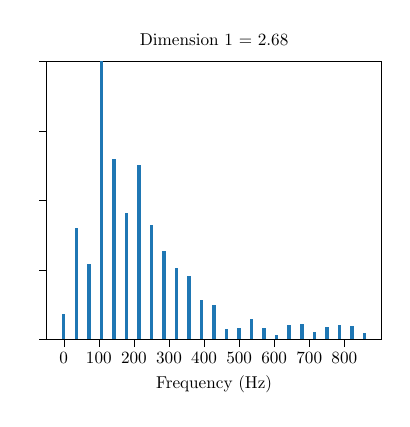
\begin{tikzpicture}[scale=0.62]

\definecolor{darkgray176}{RGB}{176,176,176}
\definecolor{steelblue31119180}{RGB}{31,119,180}

\begin{axis}[
yticklabel={\empty},
tick align=outside,
tick pos=left,
x grid style={darkgray176},
xlabel={Frequency (Hz)},
xmin=-48.3571428571429, xmax=905.5,
xtick style={color=black},
xtick={0, 100, 200, 300, 400, 500, 600, 700, 800}, % Set explicit tick positions
y grid style={darkgray176},
%ylabel={Magnitude},
ymin=0, ymax=4,
title={Dimension 1 = 2.68},
ytick style={color=black}
]
\draw[draw=none,fill=steelblue31119180] (axis cs:-5,0) rectangle (axis cs:5,0.363293109461665);
\draw[draw=none,fill=steelblue31119180] (axis cs:30.7142857142857,0) rectangle (axis cs:40.7142857142857,1.59671692845371);
\draw[draw=none,fill=steelblue31119180] (axis cs:66.4285714285714,0) rectangle (axis cs:76.4285714285714,1.08375129075336);
\draw[draw=none,fill=steelblue31119180] (axis cs:102.142857142857,0) rectangle (axis cs:112.142857142857,5.72028640718505);
\draw[draw=none,fill=steelblue31119180] (axis cs:137.857142857143,0) rectangle (axis cs:147.857142857143,2.60109171070077);
\draw[draw=none,fill=steelblue31119180] (axis cs:173.571428571429,0) rectangle (axis cs:183.571428571429,1.82230187959835);
\draw[draw=none,fill=steelblue31119180] (axis cs:209.285714285714,0) rectangle (axis cs:219.285714285714,2.50466396839656);
\draw[draw=none,fill=steelblue31119180] (axis cs:245,0) rectangle (axis cs:255,1.64154431128106);
\draw[draw=none,fill=steelblue31119180] (axis cs:280.714285714286,0) rectangle (axis cs:290.714285714286,1.2779936763853);
\draw[draw=none,fill=steelblue31119180] (axis cs:316.428571428571,0) rectangle (axis cs:326.428571428571,1.02566988726104);
\draw[draw=none,fill=steelblue31119180] (axis cs:352.142857142857,0) rectangle (axis cs:362.142857142857,0.906444113984638);
\draw[draw=none,fill=steelblue31119180] (axis cs:387.857142857143,0) rectangle (axis cs:397.857142857143,0.567573738688084);
\draw[draw=none,fill=steelblue31119180] (axis cs:423.571428571429,0) rectangle (axis cs:433.571428571429,0.497884322563813);
\draw[draw=none,fill=steelblue31119180] (axis cs:459.285714285714,0) rectangle (axis cs:469.285714285714,0.143370970638671);
\draw[draw=none,fill=steelblue31119180] (axis cs:495,0) rectangle (axis cs:505,0.158030205491621);
\draw[draw=none,fill=steelblue31119180] (axis cs:530.714285714286,0) rectangle (axis cs:540.714285714286,0.287791882784369);
\draw[draw=none,fill=steelblue31119180] (axis cs:566.428571428571,0) rectangle (axis cs:576.428571428571,0.164560600100172);
\draw[draw=none,fill=steelblue31119180] (axis cs:602.142857142857,0) rectangle (axis cs:612.142857142857,0.0653538748355305);
\draw[draw=none,fill=steelblue31119180] (axis cs:637.857142857143,0) rectangle (axis cs:647.857142857143,0.209706204538538);
\draw[draw=none,fill=steelblue31119180] (axis cs:673.571428571429,0) rectangle (axis cs:683.571428571429,0.216581742305538);
\draw[draw=none,fill=steelblue31119180] (axis cs:709.285714285714,0) rectangle (axis cs:719.285714285714,0.104565114650486);
\draw[draw=none,fill=steelblue31119180] (axis cs:745,0) rectangle (axis cs:755,0.18370350932939);
\draw[draw=none,fill=steelblue31119180] (axis cs:780.714285714286,0) rectangle (axis cs:790.714285714286,0.206670350113575);
\draw[draw=none,fill=steelblue31119180] (axis cs:816.428571428571,0) rectangle (axis cs:826.428571428571,0.196489132073225);
\draw[draw=none,fill=steelblue31119180] (axis cs:852.142857142857,0) rectangle (axis cs:862.142857142857,0.0885177801919891);
\end{axis}

\end{tikzpicture}

	\end{subfigure}
	
	\caption{The twelfth dimension is being modified, while other dimensions are fixed at 0. Negative values cause a large spike around 100Hz while positive values fully remove the 100Hz and influences the 150Hz range instead.}
	\label{fig:interpol_dim12}
\end{figure}
